\chapter{METODOLOGI}
\label{chap:metodologi}

\section{Gambaran Umum Sistem}
\label{sec:gambaran_umum_sistem}
Penelitian ini dilatarbelakangi oleh keterbatasan sensor LiDAR dua dimensi yang umum digunakan pada robot bergerak otonom untuk navigasi lingkungan dalam ruangan. Meskipun mampu menyediakan informasi jarak secara \textit{real-time} dengan tingkat akurasi yang tinggi, LiDAR 2D hanya melakukan pemindaian pada satu bidang horizontal sehingga objek yang berada di luar bidang tersebut berpotensi tidak terdeteksi (\cite{Fagundes2024,Kibii2022}). Kondisi ini dapat menimbulkan \textit{blind-spot} vertikal yang mengurangi kualitas persepsi lingkungan dan meningkatkan risiko kolisi, khususnya terhadap objek berprofil rendah yang berada di dekat permukaan lantai.

Untuk mengatasi keterbatasan tersebut, penelitian ini mengintegrasikan kamera termal sebagai sensor pelengkap LiDAR. Informasi termal digunakan untuk mengidentifikasi area yang tidak sepenuhnya teramati oleh pemindaian laser sehingga sistem dapat memperoleh representasi lingkungan yang lebih lengkap. Pendekatan integrasi antara LiDAR dan kamera termal telah banyak digunakan untuk meningkatkan robustitas persepsi pada sistem robotika dan kendaraan otonom karena kedua sensor memiliki karakteristik pengamatan yang saling melengkapi (\cite{Choi2023,Schichler2025}). Pada penelitian ini, kedua sensor tidak digabungkan secara langsung pada tingkat data mentah, melainkan diolah menjadi indikator traversability yang menggambarkan tingkat kelayakan lintasan area di depan robot. Nilai traversability dari masing-masing sensor kemudian difusikan untuk menghasilkan informasi kondisi lingkungan yang digunakan pada proses pengambilan keputusan navigasi.

Informasi traversability hasil fusi selanjutnya dimanfaatkan dalam kerangka navigasi ber\-basis \textit{Artificial Potential Field} (APF) (\cite{Khatib1986}). Metode APF dipilih karena memiliki kompleksitas komputasi yang relatif rendah dan mampu menghasilkan respons penghindaran hambatan secara \textit{real-time}. Namun demikian, penggunaan parameter APF yang bersifat tetap sering kali menyebabkan perilaku navigasi kurang adaptif terhadap perubahan kondisi lingkungan (\cite{Lv2024}). Oleh karena itu, penelitian ini memanfaatkan logika fuzzy Mamdani sebagai mekanisme adaptasi parameter navigasi berdasarkan kondisi lingkungan yang diamati sensor. Variabel masukan yang digunakan terdiri atas jarak obstacle terdekat dan nilai traversability efektif hasil fusi sensor, sedangkan keluaran fuzzy berupa skala kecepatan (\textit{speed scale}) dan penguatan gaya tolak (\textit{repulsive gain}) yang digunakan untuk menyesuaikan perilaku APF secara dinamis. Pendekatan serupa telah dilaporkan mampu meningkatkan keamanan dan kelancaran navigasi robot bergerak pada lingkungan yang kompleks (\cite{Haider2022,Benaicha2026}).

Pengembangan dan pengujian sistem dilakukan pada lingkungan simulasi berbasis ROS Noetic dan Gazebo. Penggunaan simulasi dipilih untuk menjamin reproduktivitas eksperimen, mempermudah pengendalian variabel pengujian, serta memungkinkan pelaksanaan percobaan berulang pada kondisi yang identik (\cite{Adiuku2024}). Lokalisasi robot diperoleh melalui \textit{fake\_localization} sehingga posisi robot terhadap peta diketahui secara langsung dan tidak dipengaruhi oleh kesalahan estimasi lokalisasi. Dengan demikian, evaluasi dapat difokuskan pada kinerja sistem navigasi dan kemampuan penghindaran obstacle tanpa dipengaruhi oleh ketidakpastian proses lokalisasi.

Secara umum, penelitian ini dilaksanakan melalui lima tahapan utama yang ditunjukkan pada Gambar~\ref{fig:alur_penelitian}. Tahap pertama adalah studi pendahuluan yang mencakup kajian literatur, identifikasi permasalahan, dan penetapan ruang lingkup penelitian. Tahap kedua adalah perancangan sistem yang meliputi penyusunan arsitektur navigasi, perancangan mekanisme fusi traversability, serta perancangan logika fuzzy Mamdani. Tahap ketiga adalah implementasi seluruh komponen sistem pada lingkungan simulasi. Tahap keempat adalah pelaksanaan eksperimen pada delapan skenario pengujian yang terdiri atas konfigurasi \textit{baseline} dan konfigurasi fuzzy. Tahap terakhir adalah analisis hasil eksperimen menggunakan metrik navigasi yang telah ditentukan untuk mengevaluasi pengaruh integrasi kamera termal, fusi traversability, dan logika fuzzy terhadap performa sistem navigasi robot.

\begin{figure}[H]
\centering
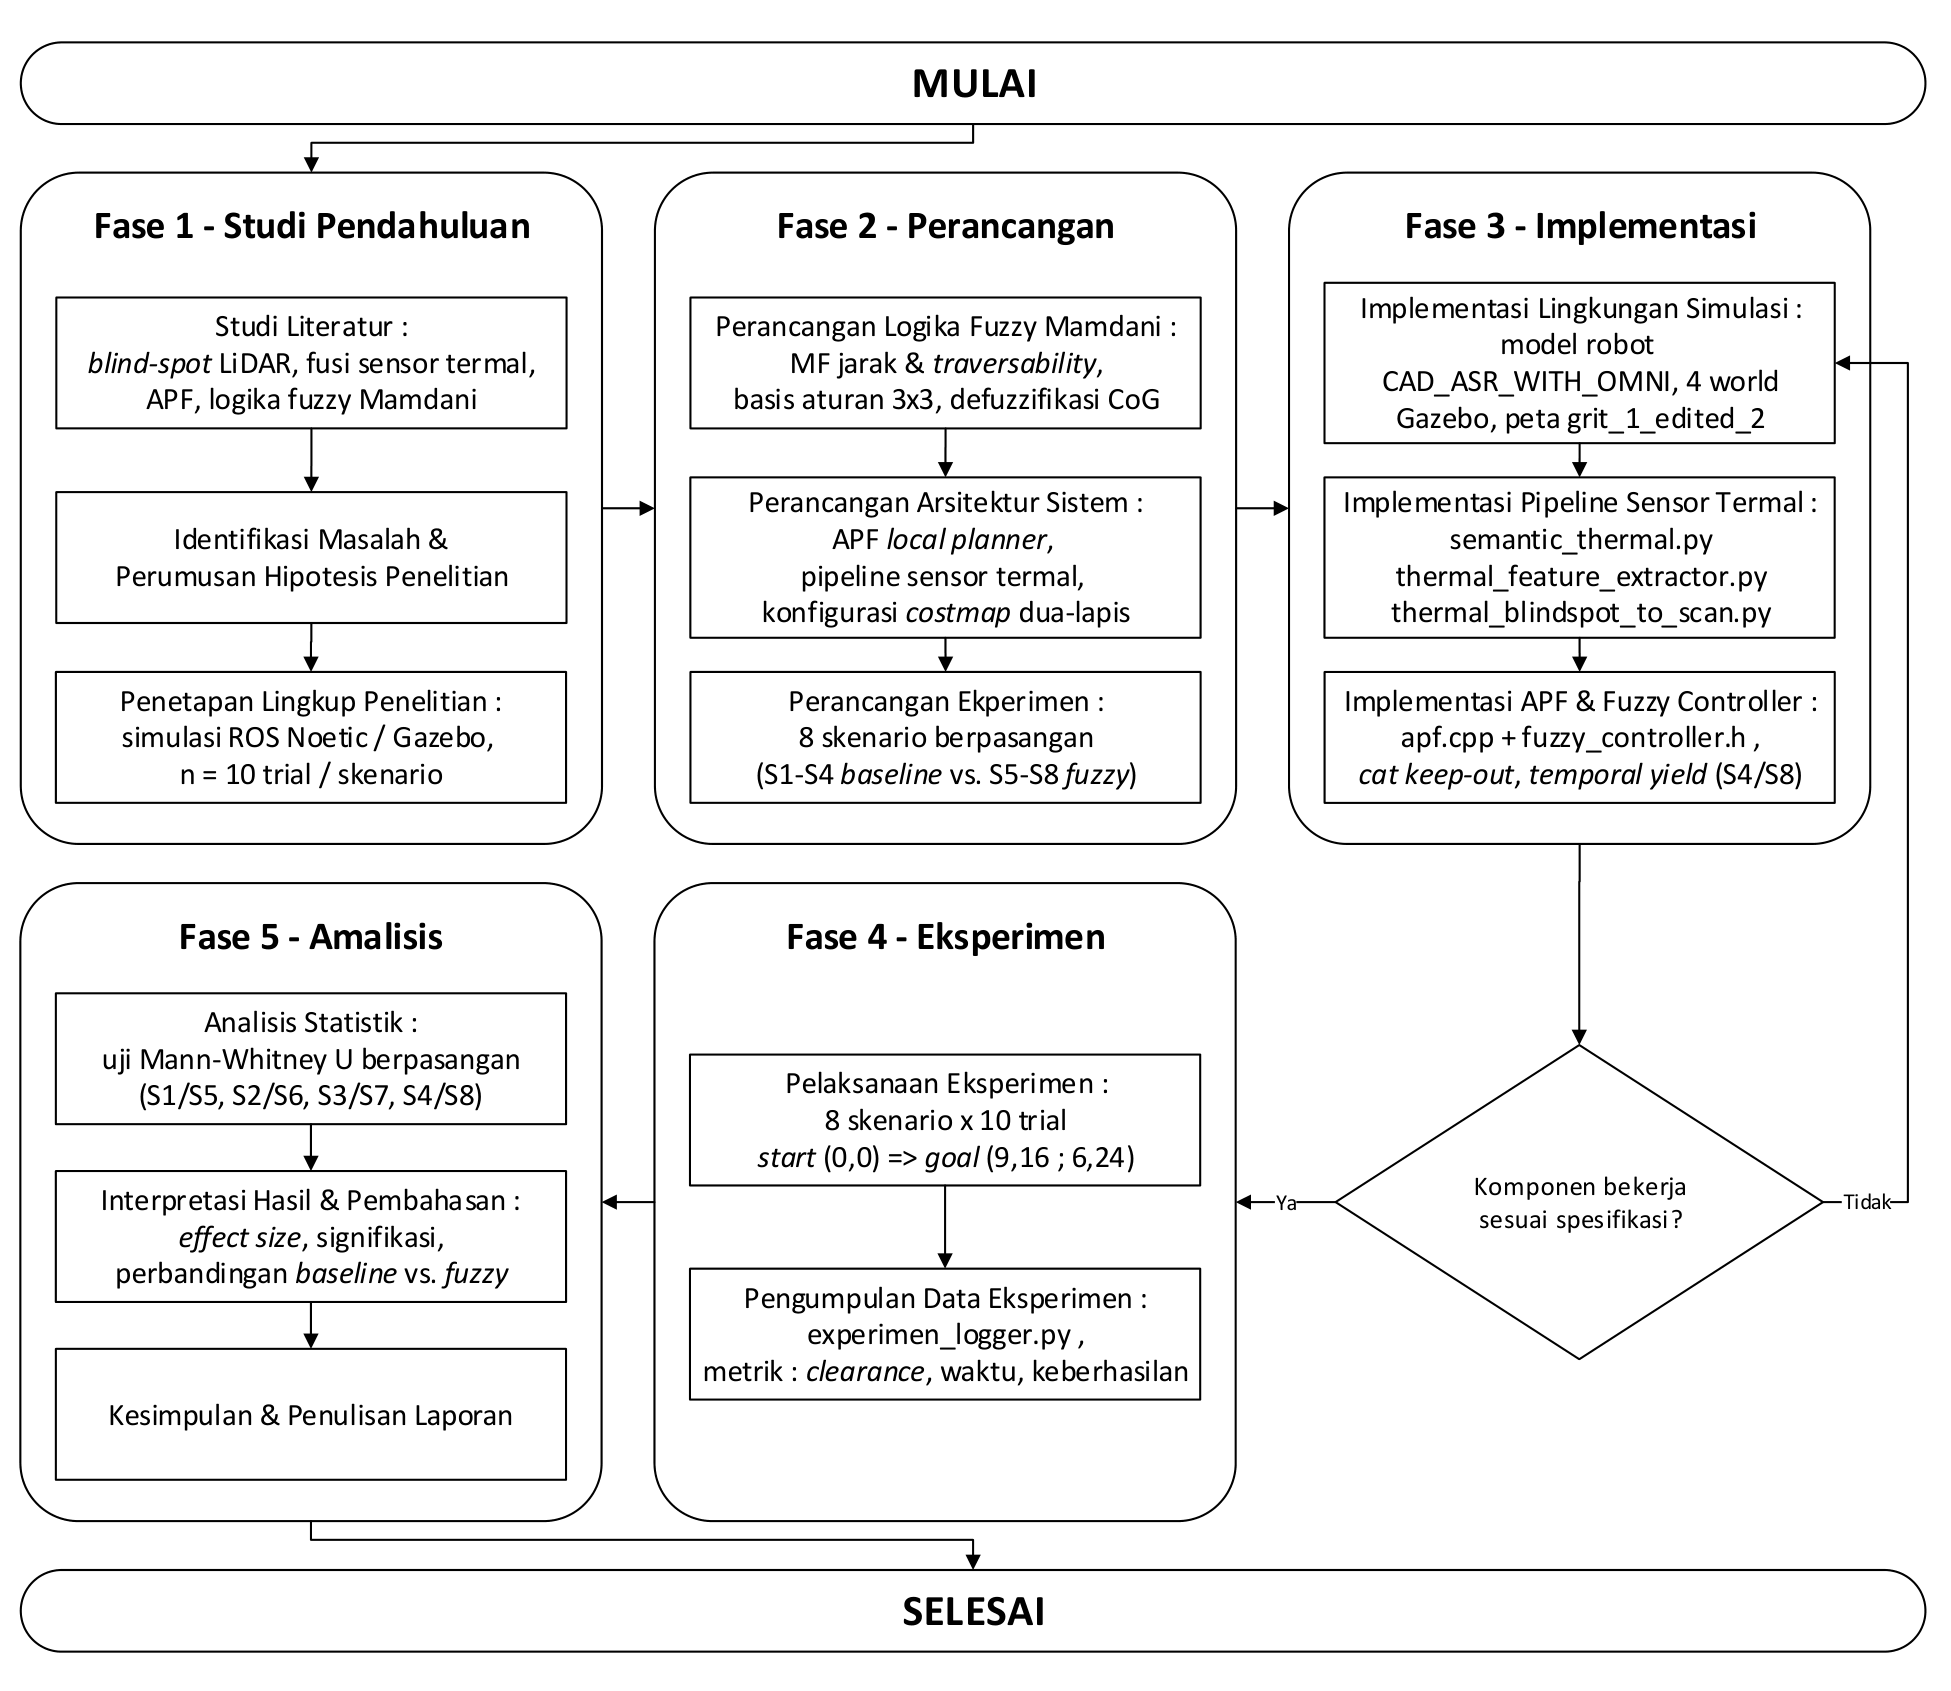
\includegraphics[width=\textwidth]{gambar/3.1_alur_penelitian.png}
\caption{Alur penelitian yang digunakan pada penelitian ini.}
\label{fig:alur_penelitian}
\end{figure}


\section{Perangkat dan Lingkungan Penelitian}
\label{sec:perangkat_dan_lingkungan}
Penelitian ini dilaksanakan sepenuhnya pada lingkungan simulasi berbasis Robot Operating System (ROS) dan Gazebo. Pendekatan simulasi dipilih untuk menjamin reproduktivitas eksperimen, memudahkan pengendalian variabel pengujian, serta memungkinkan pelaksanaan pengujian berulang pada kondisi yang identik (\cite{Adiuku2024}). Lingkungan simulasi yang digunakan dirancang untuk merepresentasikan skenario navigasi robot bergerak otonom pada area dalam ruangan dengan berbagai konfigurasi obstacle statis maupun dinamis. Subbab ini menjelaskan perangkat keras, perangkat lunak, serta lingkungan simulasi yang digunakan selama penelitian.

\subsection{Perangkat Keras}
\label{sec:perangkat_keras}

Meskipun penelitian ini tidak melibatkan robot fisik secara langsung, proses simulasi tetap memerlukan sumber daya komputasi yang memadai untuk menjalankan simulator, sistem navigasi, dan pemrosesan data sensor secara \textit{real-time}. Selain itu, model sensor yang digunakan dalam simulasi dirancang untuk merepresentasikan karakteristik sensor yang umum digunakan pada robot bergerak otonom.

\subsubsection*{a. Komputer Host}

Seluruh simulasi dan pengolahan data dilakukan pada komputer host dengan spesifikasi yang disajikan pada Tabel~\ref{tab:spesifikasi_komputer_host}. Spesifikasi tersebut dinilai memadai untuk menjalankan simulasi Gazebo, pemrosesan data sensor, serta pencatatan data eksperimen secara bersamaan selama proses pengujian berlangsung.

\begin{table}[H]
\centering
\caption{Spesifikasi komputer host yang digunakan dalam penelitian}
\label{tab:spesifikasi_komputer_host}
\begin{tabular}{ll}
\toprule
\textbf{Komponen} & \textbf{Spesifikasi} \\
\midrule
Sistem Operasi & Ubuntu 20.04 LTS (64-bit) \\
Prosesor & AMD Ryzen 5 6600H \\
RAM & 16 GB \\
GPU & NVIDIA GeForce RTX 3050 Laptop GPU (4 GB VRAM) \\
\bottomrule
\end{tabular}
\end{table}

\subsubsection*{b. Model Robot}

Robot yang digunakan dalam penelitian ini adalah \texttt{CAD\_ASR\_WITH\_OMNI}, yaitu robot be\-roda tiga dengan konfigurasi omnidirectional (holonomik) yang memungkinkan robot bergerak ke berbagai arah tanpa harus mengubah orientasi badan robot terlebih dahulu. Model robot didefinisikan menggunakan \textit{Unified Robot Description Format} (URDF) dan dijalankan pada lingkungan simulasi Gazebo melalui antarmuka ROS (\cite{Adiuku2024}).

Untuk keperluan navigasi, robot direpresentasikan menggunakan \textit{footprint} berbentuk per\-segi dengan dimensi 0,54 m $\times$ 0,64 m. Representasi \textit{footprint} tersebut digunakan oleh sistem \textit{costmap} untuk menentukan ruang bebas, memperhitungkan jarak aman terhadap obstacle, serta mendukung proses perencanaan lintasan selama navigasi berlangsung.

\subsubsection*{c. Sensor LiDAR}

Sensor utama yang digunakan dalam penelitian ini adalah LiDAR dua dimensi yang menghasilkan data pindaian lingkungan dalam format \texttt{sensor\_msgs/LaserScan}. Sensor ini memiliki cakupan sudut horizontal sebesar 360$^\circ$ dengan frekuensi pembaruan 40 Hz dan digunakan sebagai sumber utama informasi geometris lingkungan.

Data LiDAR dimanfaatkan untuk mendeteksi obstacle, menghitung jarak terhadap obstacle terdekat, serta mendukung proses perencanaan lintasan robot. Namun demikian, LiDAR dua dimensi hanya melakukan pemindaian pada satu bidang horizontal sehingga memiliki keterbatasan dalam mendeteksi obstacle yang seluruh profilnya berada di luar bidang pindai sensor. Keterbatasan tersebut menyebabkan munculnya area \textit{blind-spot} yang menjadi salah satu permasalahan utama pada penelitian ini (\cite{Fagundes2024,Kibii2022}).

\subsubsection*{d. Kamera Termal}

Selain LiDAR, penelitian ini menggunakan kamera termal sebagai sensor pelengkap untuk meningkatkan kemampuan persepsi lingkungan. Kamera termal menghasilkan citra berbasis distribusi intensitas panas yang direpresentasikan dalam format \textit{grayscale}. Berbeda dengan LiDAR yang mengandalkan informasi geometris, kamera termal mampu mengidentifikasi objek berdasarkan karakteristik termalnya sehingga tetap dapat mendeteksi obstacle tertentu yang tidak teramati oleh LiDAR (\cite{Choi2023}).

Informasi yang diperoleh dari kamera termal digunakan untuk mengestimasi kondisi area di depan robot serta mendukung proses pembentukan informasi traversability lingkungan. Pendekatan integrasi LiDAR dan kamera termal banyak digunakan pada sistem robotika modern karena kedua sensor memiliki karakteristik pengamatan yang saling melengkapi (\cite{Schichler2025}).

Spesifikasi sensor yang digunakan dalam simulasi ditunjukkan pada Tabel~\ref{tab:spesifikasi_sensor}.

\begin{table}[H]
\centering
\caption{Spesifikasi sensor yang digunakan dalam simulasi}
\label{tab:spesifikasi_sensor}
\begin{tabular}{llll}
\toprule
\textbf{Parameter} & \textbf{LiDAR} & \textbf{Kamera Termal} & \textbf{Satuan} \\
\midrule
Frame pemasangan & laser & thermal\_link & -- \\
Posisi dari base\_link (x, y) & (0,147; 0,362) & (0,170; 0,660) & m \\
Orientasi yaw & 0 & -0,52 & rad \\
Cakupan sudut horizontal & 360$^\circ$ & 90$^\circ$ & -- \\
Resolusi data & 720 sampel & 640 $\times$ 480 & -- \\
Jangkauan minimum & 0,05 & 0,10 & m \\
Jangkauan maksimum & 12,0 & 100,0 & m \\
Frekuensi pembaruan & 40 & 10 & Hz \\
Keluaran data & LaserScan & Citra termal grayscale & -- \\
\bottomrule
\end{tabular}
\end{table}

\subsection{Perangkat Lunak}
\label{sec:perangkat_lunak}

Pengembangan sistem dilakukan menggunakan beberapa perangkat lunak yang saling terintegrasi dalam ekosistem ROS. Daftar perangkat lunak dan modul utama yang digunakan dalam penelitian ini disajikan pada Tabel~\ref{tab:perangkat_lunak}.

\begin{table}[H]
\centering
\caption{Perangkat lunak dan modul utama yang digunakan}
\label{tab:perangkat_lunak}
\begin{tabular}{p{3.5cm}p{2cm}p{7cm}}
\toprule
\textbf{Komponen} & \textbf{Versi} & \textbf{Fungsi} \\
\midrule
Ubuntu & 20.04 LTS & Sistem operasi host \\
ROS Noetic & Noetic & Middleware komunikasi sistem \\
Gazebo & 11 & Simulator robot dan lingkungan \\
NavfnROS & 1.17.3 & Perencanaan lintasan global \\
APFPlanner & Kustom & Perencanaan lintasan lokal \\
OpenCV & 4.2.0 & Pemrosesan citra termal \\
semantic\-\_thermal.py & Kustom & Segmentasi citra termal \\
thermal\_feature\-\_extractor.py & Kustom & Ekstraksi fitur traversability \\
thermal\_blindspot\-\_to\_scan.py & Kustom & Pembentukan \textit{virtual scan} termal \\
experiment\-\_logger.py & Kustom & Pencatatan data eksperimen \\
\bottomrule
\end{tabular}
\end{table}

ROS Noetic digunakan sebagai \textit{middleware} yang menghubungkan seluruh komponen sistem melalui mekanisme komunikasi berbasis topik. Sementara itu, Gazebo berperan sebagai simulator yang menyediakan lingkungan virtual, model robot, serta emulasi sensor yang digunakan selama proses pengujian. Integrasi ROS dan Gazebo banyak digunakan dalam penelitian robotika karena mendukung pengembangan sistem secara modular dan reproduktif (\cite{Macenski2022,Adiuku2024}).

Selain perangkat lunak utama, penelitian ini juga memanfaatkan beberapa pustaka pendukung seperti NumPy untuk komputasi numerik, OpenCV untuk pemrosesan citra, Pandas untuk pengelolaan data eksperimen, serta SciPy untuk analisis statistik hasil pengujian.

\subsection{Lingkungan Simulasi}
\label{sec:lingkungan_simulasi}

\subsubsection*{a. Model Robot \texttt{CAD\_ASR\_WITH\_OMNI}}

Lingkungan simulasi menggunakan model robot \texttt{CAD\_ASR\_WITH\_OMNI} yang telah dileng\-kapi dengan sensor LiDAR dan kamera termal. Kedua sensor ditempatkan pada bagian depan robot untuk memaksimalkan area pengamatan ke arah pergerakan robot. Visualisasi model robot dan posisi pemasangan sensor ditunjukkan pada Gambar~\ref{fig:model_robot_sensor}.

\begin{figure}[H]
\centering
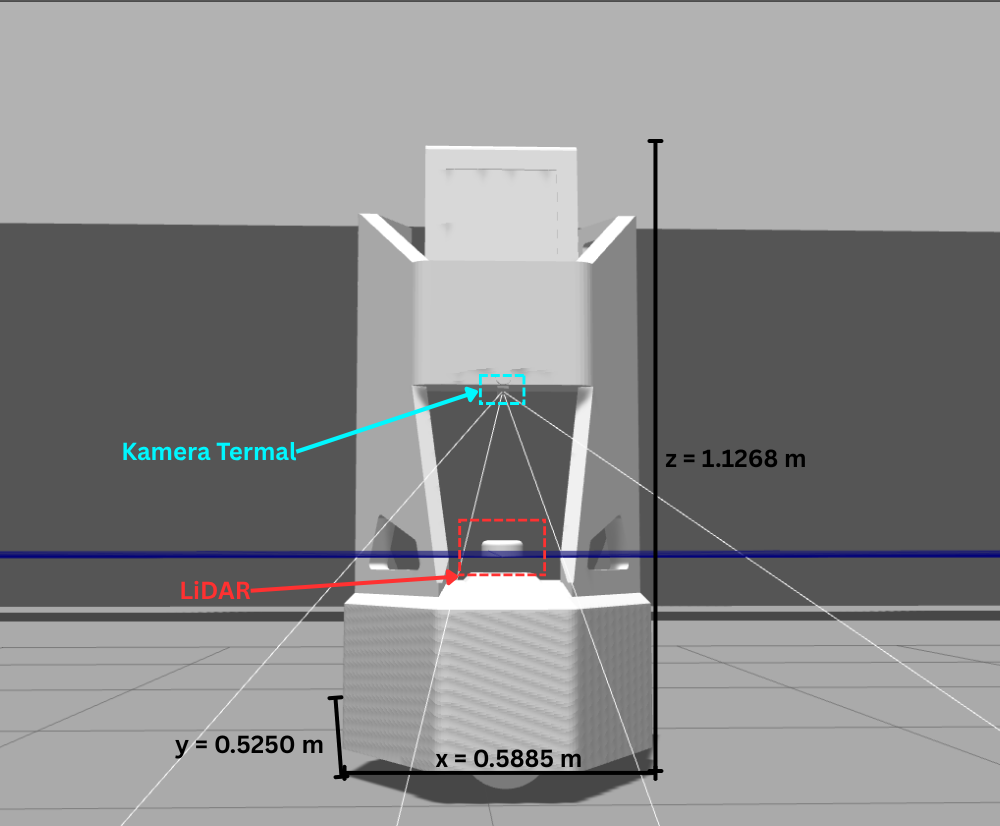
\includegraphics[width=0.5\textwidth]{gambar/3.2_robot_model.png}
\caption{Model robot \texttt{CAD\_ASR\_WITH\_OMNI} dan penempatan sensor.}
\label{fig:model_robot_sensor}
\end{figure}

\subsubsection*{b. Peta Lingkungan Simulasi}

Navigasi robot dilakukan pada lingkungan dalam ruangan yang direpresentasikan menggunakan \textit{occupancy grid map}. Peta disediakan melalui paket \textit{map\_server} dan digunakan oleh \textit{global planner} untuk menghasilkan lintasan menuju tujuan.

Peta yang digunakan pada penelitian ini adalah \texttt{grit\_1\_edited\_2}, yang memuat informasi area bebas, area terhalang, dan batas lingkungan simulasi. Representasi peta tersebut menjadi dasar pembentukan \textit{global costmap} yang digunakan oleh sistem navigasi.

\subsubsection*{c. Lokalisasi Robot}

Lokalisasi robot dilakukan menggunakan komponen \textit{fake\_localization}, yaitu metode loka\-lisasi yang memanfaatkan posisi \textit{ground-truth} dari simulator Gazebo sebagai estimasi pose robot pada peta. Pendekatan ini dipilih karena penelitian berfokus pada evaluasi sistem navigasi dan penghindaran obstacle, bukan pada akurasi estimasi posisi robot.

Dengan menggunakan \textit{fake\_localization}, pengaruh kesalahan lokalisasi dapat dieliminasi sehingga perbedaan performa yang diamati antara konfigurasi pengujian berasal dari meka\-nisme navigasi yang digunakan, bukan dari ketidakpastian estimasi posisi robot.

\subsubsection*{d. Obstacle Pengujian}

Penelitian ini menggunakan beberapa jenis obstacle yang ditempatkan pada lingkungan simulasi untuk merepresentasikan kondisi navigasi yang berbeda. Karakteristik obstacle yang digunakan disajikan pada Tabel~\ref{tab:spesifikasi_obstacle}.

\begin{table}[H]
\centering
\caption{Spesifikasi obstacle yang digunakan dalam simulasi}
\label{tab:spesifikasi_obstacle}
\begin{tabular}{llll}
\toprule
\textbf{Nama Model} & \textbf{Jenis} & \textbf{Radius} & \textbf{Terdeteksi LiDAR} \\
\midrule
obstacle\_cat & Statis & 0,18 m & Tidak \\
obstacle\_human\_1 & Statis/Dinamis & 0,25 m & Ya \\
obstacle\_human\_2 & Statis/Dinamis & 0,25 m & Ya \\
obstacle & Statis & 0,25 m & Ya \\
\bottomrule
\end{tabular}
\end{table}

Obstacle \texttt{obstacle\_cat} digunakan untuk merepresentasikan obstacle berprofil rendah yang berada pada area \textit{blind-spot} LiDAR. Sebaliknya, obstacle manusia dan obstacle umum memiliki dimensi yang cukup tinggi sehingga dapat dideteksi secara langsung oleh sensor LiDAR. Pada skenario dinamis, obstacle manusia digerakkan secara periodik untuk mensimulasikan keberadaan objek bergerak pada lingkungan navigasi robot.

\section{Arsitektur Sistem}
\label{sec:arsitektur}

\subsection{Diagram Arsitektur Sistem}

Arsitektur sistem navigasi yang diusulkan dirancang untuk mengintegrasikan informasi geometris dari sensor LiDAR dengan informasi termal dari kamera termal dalam satu kerangka pengambilan keputusan navigasi. Sistem dibangun menggunakan pendekatan modular berbasis Robot Operating System (ROS), sehingga setiap fungsi direalisasikan sebagai node yang saling bertukar data melalui mekanisme publish--subscribe (\cite{Macenski2022}).

Berbeda dengan pendekatan navigasi konvensional yang hanya memanfaatkan informasi jarak dari LiDAR, penelitian ini memperkenalkan mekanisme fusi traversability yang menggabungkan hasil persepsi dari kedua sensor untuk membentuk representasi kondisi lingkungan yang lebih komprehensif. Informasi tersebut selanjutnya digunakan oleh pengendali fuzzy Mamdani untuk menyesuaikan perilaku navigasi berbasis Artificial Potential Field (APF) secara adaptif.

Arsitektur keseluruhan sistem ditunjukkan pada Gambar~\ref{fig:arsitektur_pipeline}.

\begin{figure}[H]
    \centering
    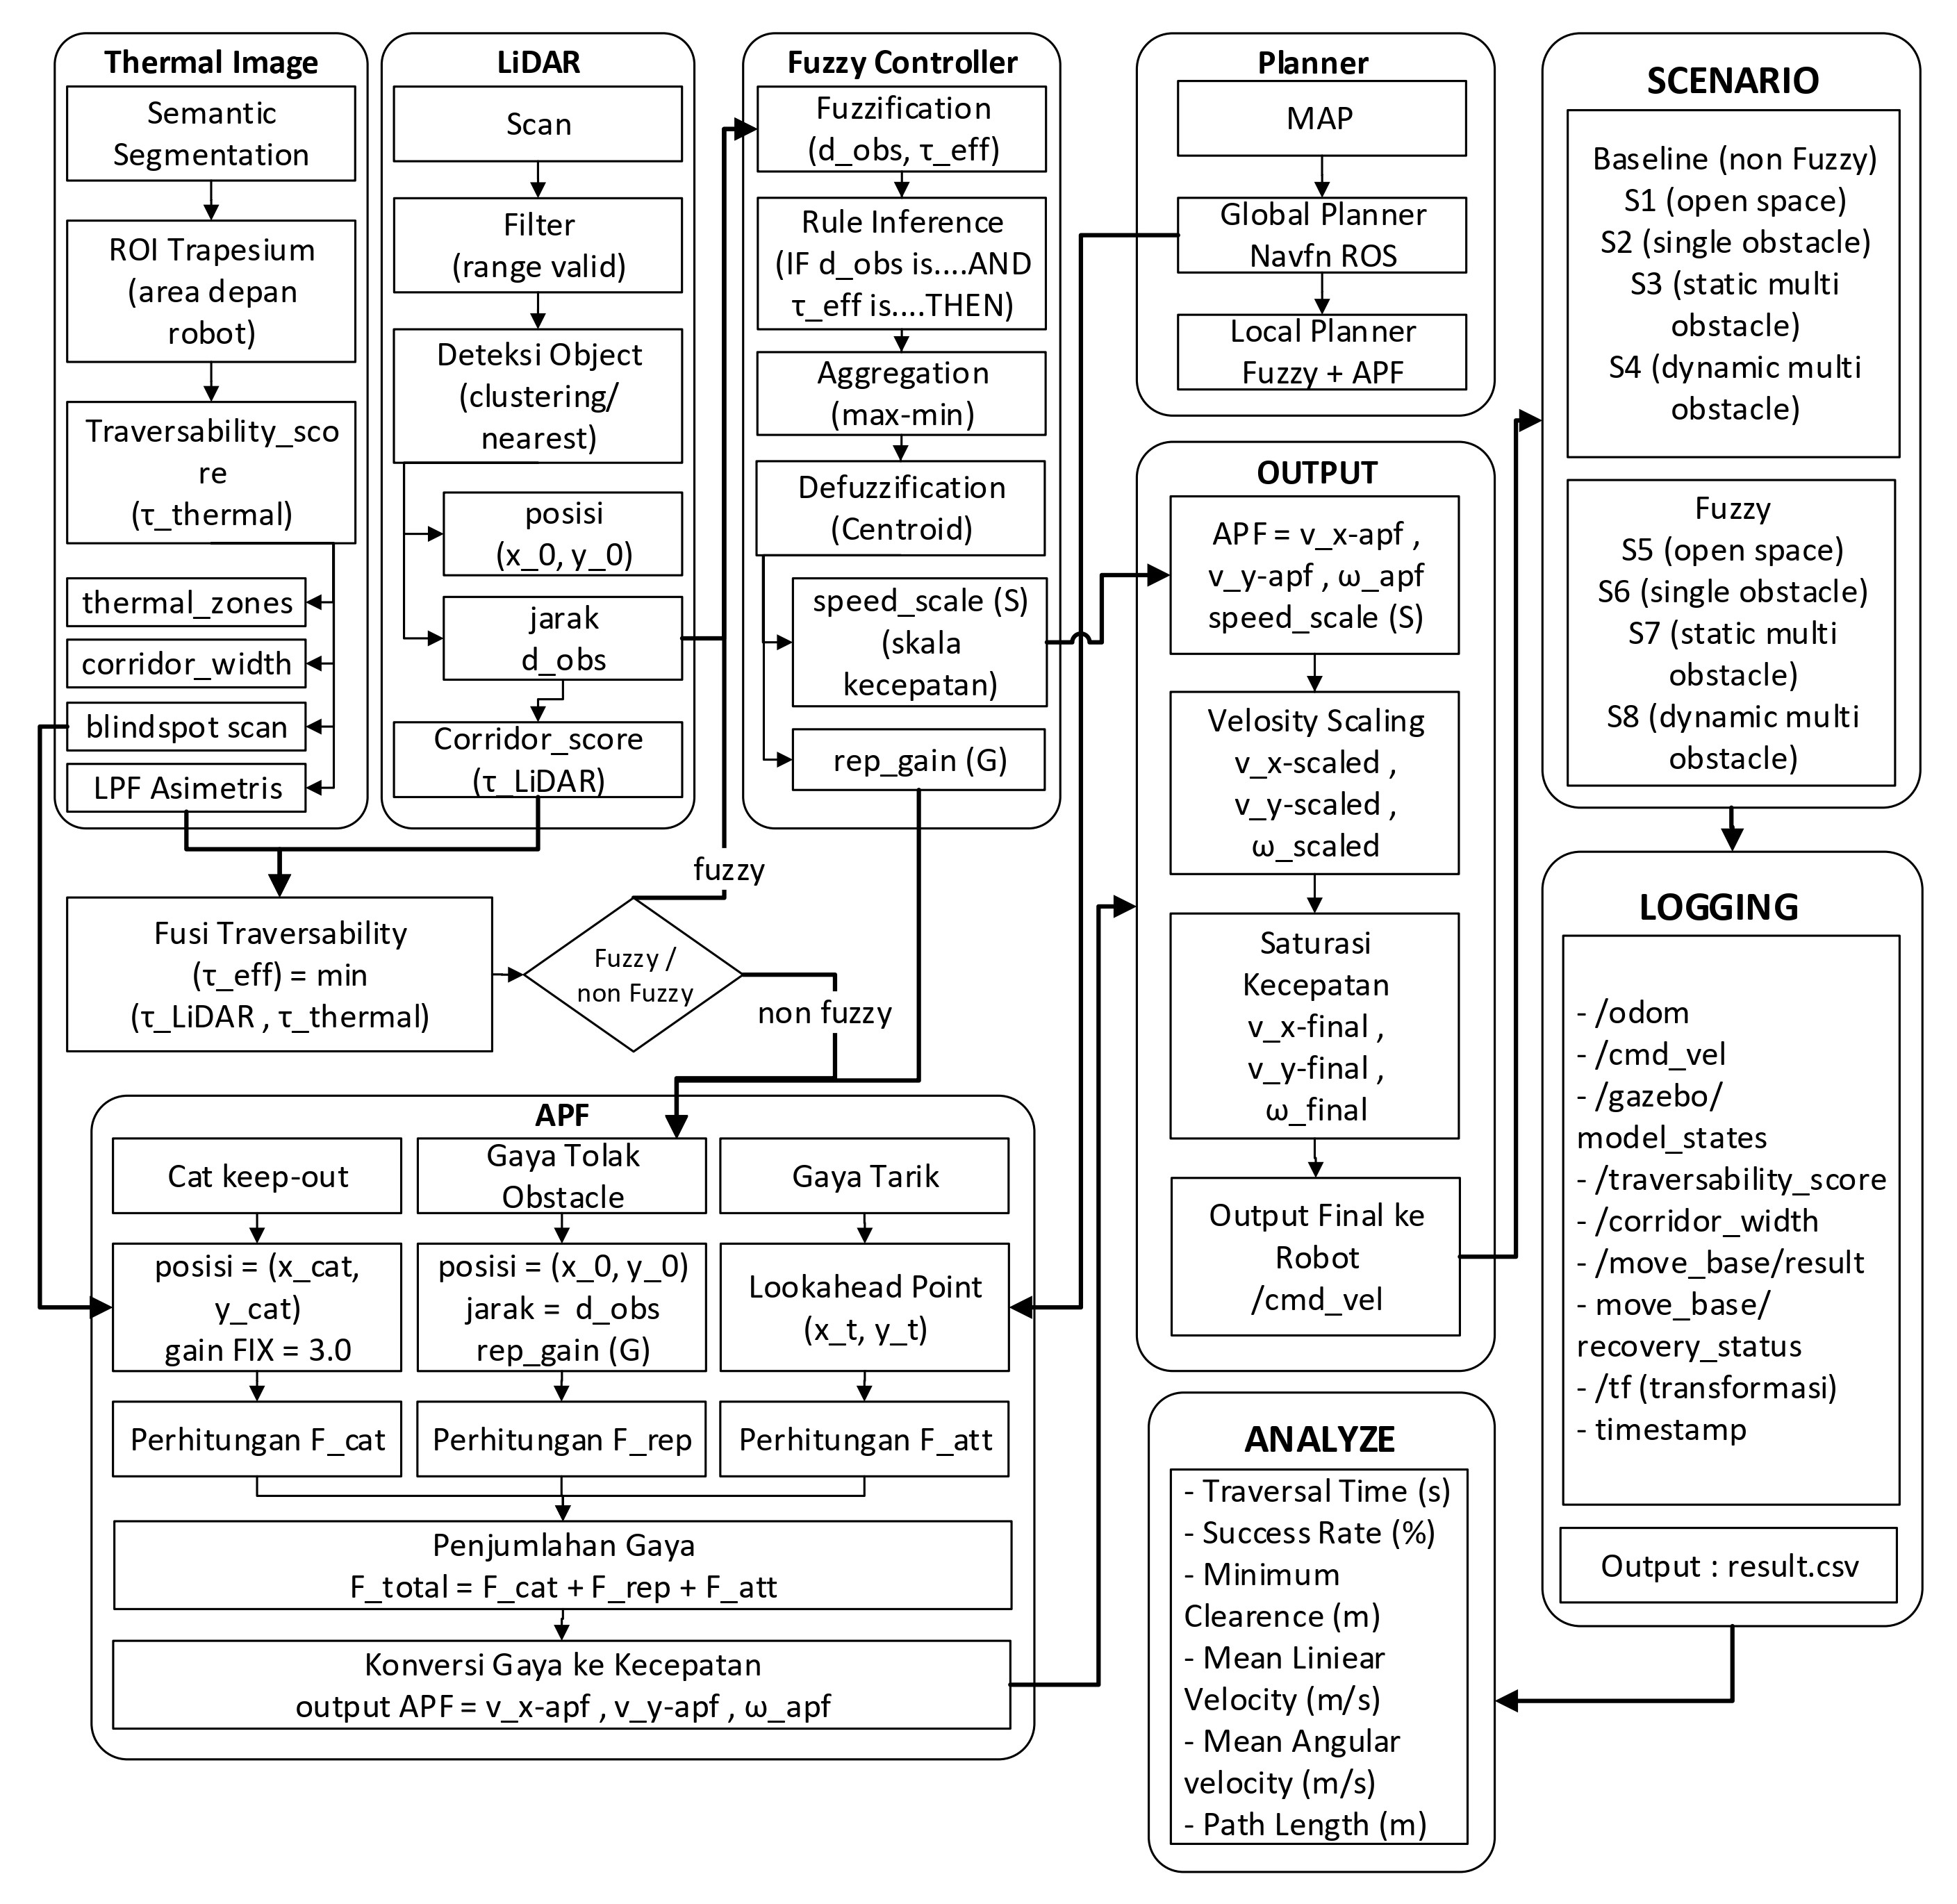
\includegraphics[width=0.7\textwidth]{gambar/3.3_arsitektur_pipeline.jpg}
    \caption{Arsitektur sistem navigasi yang diusulkan.}
    \label{fig:arsitektur_pipeline}
\end{figure}

\subsection{Jalur Pemrosesan Kamera Termal}

Kamera termal menghasilkan citra inframerah berformat grayscale melalui topik \texttt{/the\-rmal/thermal\_camera/image\_raw}. Jalur pemrosesan termal terdiri atas tiga node utama, yaitu \texttt{semantic\_thermal.py}, \texttt{thermal\_feature\_extractor.py}, dan \texttt{thermal\_blindsp\-ot\_to\_scan.py}.

Node \texttt{semantic\_thermal.py} bertugas melakukan segmentasi semantik terhadap citra termal mentah untuk membedakan area obstacle dan area yang dapat dilalui. Hasil segmentasi kemudian diteruskan ke node \texttt{thermal\_feature\_extractor.py} untuk mengekstraksi informasi lingkungan berupa skor traversability termal, lebar koridor, serta kondisi zona navigasi pada area kiri, tengah, dan kanan.

Selain menghasilkan fitur traversability, hasil segmentasi juga digunakan oleh \texttt{thermal\-\_blindspot\_to\_scan.py} untuk membentuk virtual scan yang merepresentasikan obstacle termal pada area blind-spot LiDAR. Pendekatan ini memungkinkan obstacle yang tidak terdeteksi oleh sensor laser tetap dapat dipertimbangkan oleh sistem navigasi tanpa memerlukan perubahan struktur pada ROS Navigation Stack.

\subsection{Jalur Pemrosesan LiDAR}

Sensor LiDAR berfungsi sebagai sumber utama informasi geometris lingkungan. Data hasil pemindaian diterima melalui topik \texttt{/scan} dan digunakan untuk mendeteksi obstacle di sekitar robot serta menghitung karakteristik ruang bebas yang tersedia.

Selain digunakan untuk membangun representasi obstacle pada costmap, data LiDAR juga dimanfaatkan untuk menentukan jarak obstacle terdekat terhadap robot. Informasi tersebut menjadi salah satu variabel penting yang digunakan pada proses pengambilan keputusan navigasi.

Pada penelitian ini, data LiDAR juga digunakan untuk menghitung skor traversability berbasis geometri lingkungan. Nilai traversability tersebut menggambarkan tingkat kemudahan robot untuk bergerak berdasarkan ruang bebas yang tersedia di depan robot. Konsep traversability dipilih karena mampu merangkum kondisi lingkungan ke dalam satu indikator kuantitatif yang lebih mudah digunakan pada proses pengambilan keputusan (\cite{Sevastopoulos2022}).

\subsection{Fusi Traversability dan Pengendali Fuzzy}

Nilai traversability yang dihasilkan oleh kamera termal dan LiDAR tidak digunakan secara terpisah, melainkan digabungkan melalui mekanisme fusi traversability untuk menghasilkan nilai traversability efektif (\textit{effective traversability}). Pendekatan ini memungkinkan sistem mempertimbangkan informasi dari kedua sensor secara bersamaan sebelum mengambil keputusan navigasi.

Nilai traversability efektif selanjutnya digunakan bersama informasi jarak obstacle terdekat sebagai masukan bagi pengendali fuzzy Mamdani (\cite{Mamdani1974}). Melalui proses fuzzifikasi, evaluasi aturan, agregasi, dan defuzzifikasi, sistem menghasilkan dua parameter adaptif yang digunakan pada local planner, yaitu \textit{speed scale} dan \textit{repulsive gain}.

Parameter \textit{speed scale} digunakan untuk menyesuaikan kecepatan linear robot sesuai kondisi lingkungan yang diamati sensor. Sementara itu, parameter \textit{repulsive gain} digunakan untuk mengatur kekuatan gaya tolak obstacle pada APF. Dengan pendekatan ini, perilaku navigasi dapat beradaptasi terhadap perubahan kondisi lingkungan secara lebih fleksibel dibandingkan penggunaan parameter yang bersifat tetap (\cite{Haider2022,Benaicha2026}).

\subsection{Integrasi APF dengan ROS Navigation Stack}

Sistem navigasi yang diusulkan dibangun di atas ROS Navigation Stack yang terdiri atas \textit{map\_server}, \textit{costmap}, \textit{move\_base}, dan \textit{NavfnROS}. Komponen \textit{map\_server} menyediakan peta lingkungan dalam bentuk occupancy grid map yang digunakan sebagai dasar perencanaan lintasan global.

Perencanaan lintasan global dilakukan oleh NavfnROS menggunakan algoritma Dijkstra untuk menghasilkan jalur bebas obstacle dari posisi robot menuju titik tujuan. Jalur global tersebut selanjutnya digunakan oleh APFPlanner sebagai referensi navigasi lokal.

APFPlanner menghitung gaya tarik menuju tujuan dan gaya tolak terhadap obstacle berd\-asarkan informasi yang diperoleh dari sensor. Sebelum dikonversi menjadi perintah kecepatan robot, parameter gaya tolak dan kecepatan linear terlebih dahulu disesuaikan menggunakan keluaran pengendali fuzzy. Hasil akhir proses ini dipublikasikan melalui topik \texttt{/cmd\_vel} dan digunakan untuk menggerakkan robot pada lingkungan simulasi.

\subsection{Konfigurasi Baseline dan Fuzzy}

Untuk mengevaluasi pengaruh pengendali fuzzy terhadap performa navigasi, penelitian ini menggunakan dua konfigurasi sistem yang diuji pada kondisi lingkungan yang identik. Konfigurasi pertama adalah sistem baseline, sedangkan konfigurasi kedua adalah sistem yang dilengkapi mekanisme adaptasi berbasis logika fuzzy.

\begin{table}[H]
\centering
\caption{Kelompok skenario pengujian}
\label{tab:kelompok_skenario}
\begin{tabular}{ll}
\toprule
Kelompok & Skenario \\
\midrule
Baseline & S1, S2, S3, S4 \\
Fuzzy & S5, S6, S7, S8 \\
\bottomrule
\end{tabular}
\end{table}

Pada kedua konfigurasi, sensor LiDAR dan kamera termal tetap diaktifkan sehingga informasi lingkungan yang digunakan sistem bersifat identik. Perbedaan utama terletak pada mekanisme pengendalian yang diterapkan pada APFPlanner.

Konfigurasi baseline menggunakan parameter navigasi yang bersifat tetap, sedangkan konfigurasi fuzzy menggunakan inferensi Mamdani untuk menyesuaikan skala kecepatan dan penguatan gaya tolak berdasarkan kombinasi jarak obstacle dan traversability hasil fusi sensor. Dengan konfigurasi tersebut, pengaruh logika fuzzy terhadap performa navigasi dapat dievaluasi secara langsung tanpa dipengaruhi oleh perubahan konfigurasi sensor maupun lingkungan pengujian.



\section{Pemrosesan LiDAR}
\label{sec:pemrosesan_lidar}
Sensor LiDAR berperan sebagai sumber utama informasi geometris lingkungan dalam sistem navigasi yang diusulkan. Data hasil pemindaian digunakan untuk mendeteksi obstacle di sekitar robot, mengukur jarak terhadap obstacle terdekat, serta mengestimasi tingkat keterlaluan (\textit{traversability}) area di depan robot. Informasi tersebut selanjutnya digunakan pada proses fusi sensor dan pengambilan keputusan navigasi.

Berbeda dengan kamera termal yang menghasilkan representasi lingkungan dalam bentuk citra, LiDAR menghasilkan data jarak yang bersifat langsung dan memiliki ketelitian spasial yang tinggi. Oleh karena itu, sensor ini tetap menjadi komponen utama dalam proses perencanaan lintasan dan penghindaran obstacle pada penelitian ini (\cite{Fagundes2024,Liu2024}).

\subsection{Akuisisi Data LiDAR}

Sensor LiDAR menghasilkan data pindaian dalam format \texttt{sensor\_msgs/LaserScan} y\-ang dipublikasikan melalui topik \texttt{/scan}. Data tersebut terdiri atas sekumpulan pasangan sudut dan jarak yang merepresentasikan obstacle pertama yang terdeteksi pada setiap arah pengamatan.

Pada penelitian ini, sensor LiDAR memiliki cakupan pemindaian horizontal sebesar 360$^\circ$ dengan frekuensi pembaruan 40 Hz. Setiap siklus pemindaian menghasilkan 720 sampel jarak yang mencakup seluruh area di sekitar robot. Data tersebut digunakan secara simultan oleh ROS Navigation Stack dan APFPlanner untuk membangun representasi lingkungan lokal.

\subsection{Keterbatasan Blind-Spot Vertikal LiDAR}

Meskipun mampu memberikan informasi jarak secara akurat, LiDAR dua dimensi memiliki keterbatasan inheren karena hanya melakukan pemindaian pada satu bidang horizontal dengan ketinggian tetap terhadap lantai. Akibatnya, obstacle yang seluruh profilnya berada di bawah bidang pindai tidak akan menghasilkan pantulan laser dan tidak dapat dideteksi oleh sensor (\cite{Kibii2022,Fagundes2024}).

Secara konseptual, suatu obstacle hanya dapat dideteksi apabila sebagian profil objek memotong bidang pindai LiDAR. Jika seluruh bagian obstacle berada di bawah bidang tersebut, maka obstacle akan berada pada area \textit{blind-spot}. Kondisi ini umum dijumpai pada robot bergerak yang menggunakan LiDAR dua dimensi untuk navigasi dalam ruangan, khususnya ketika berhadapan dengan obstacle berprofil rendah seperti hewan peliharaan, benda kecil di lantai, atau objek yang memiliki tinggi lebih rendah dibandingkan posisi sensor.

Pada penelitian ini, kondisi tersebut direpresentasikan melalui obstacle kucing (\texttt{obstac\-le\_cat}) yang memiliki tinggi lebih rendah dibandingkan bidang pindai LiDAR. Akibatnya, obstacle tersebut tidak dapat terdeteksi oleh sensor laser meskipun berada tepat pada jalur pergerakan robot. Keterbatasan inilah yang menjadi dasar penggunaan kamera termal sebagai sensor pelengkap untuk meningkatkan kemampuan persepsi lingkungan.

\begin{figure}[H]
\centering
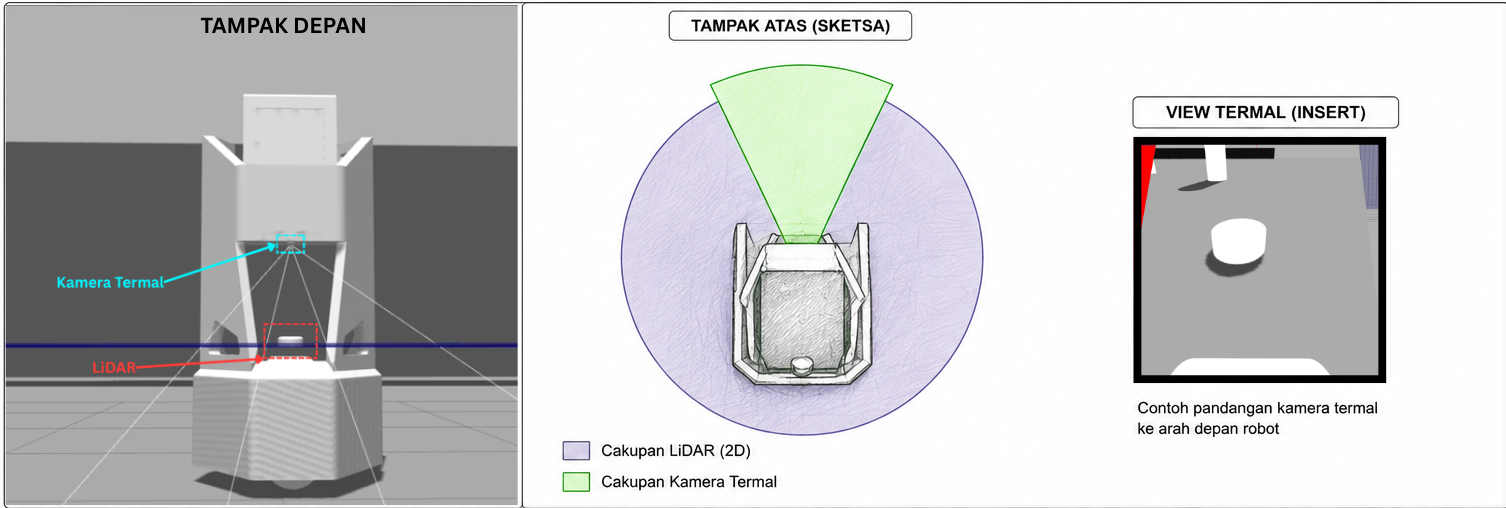
\includegraphics[width=0.85\textwidth]{gambar/3.4_lidar_thermal_fov.png}
\caption{Ilustrasi blind-spot vertikal pada sensor LiDAR dua dimensi.}
\label{fig:lidar_blindspot}
\end{figure}

\subsection{Deteksi Obstacle Terdekat}

Selain digunakan untuk membangun costmap, data LiDAR juga dimanfaatkan secara langsung oleh APFPlanner untuk menentukan jarak obstacle terdekat terhadap robot. Informasi ini diperlukan karena gaya tolak pada Artificial Potential Field bergantung pada jarak relatif antara robot dan obstacle.

Proses deteksi dilakukan dengan mencari nilai jarak minimum yang masih berada dalam rentang valid sensor. Misalkan himpunan data LiDAR dinyatakan sebagai

\begin{equation}
D = \{d_1,d_2,\dots,d_n\}
\end{equation}

maka jarak obstacle terdekat dapat diperoleh melalui

\begin{equation}
d_{obs} = \min(D)
\label{eq:min_obs_distance}
\end{equation}

dengan:

\begin{itemize}
\item $d_{obs}$ adalah jarak obstacle terdekat terhadap robot (m),
\item $D$ adalah himpunan data jarak valid dari LiDAR.
\end{itemize}

Nilai $d_{obs}$ selanjutnya digunakan sebagai salah satu variabel masukan pada pengendali fuzzy yang akan dibahas pada Subbab~\ref{sec:fuzzy_Aapf}.

\subsection{Estimasi Traversability Berbasis LiDAR}

Selain menghasilkan informasi jarak obstacle, data LiDAR juga digunakan untuk mengestimasi tingkat keterlaluan area di depan robot. Konsep traversability digunakan untuk mengg\-ambarkan seberapa aman suatu area untuk dilalui berdasarkan ruang bebas yang tersedia (\cite{Sevastopoulos2022}).

Pada penelitian ini, estimasi traversability LiDAR dilakukan dengan memanfaatkan informasi lebar koridor bebas di sekitar arah pergerakan robot. Semakin besar ruang bebas yang tersedia, semakin tinggi nilai traversability yang dihasilkan.

Lebar koridor bebas dinyatakan sebagai

\begin{equation}
w_{free}=x_{right}-x_{left}
\label{eq:free_width}
\end{equation}

dengan:

\begin{itemize}
\item $x_{right}$ adalah batas kanan area bebas,
\item $x_{left}$ adalah batas kiri area bebas.
\end{itemize}

Nilai traversability LiDAR kemudian dinormalisasi ke rentang $[0,1]$ sehingga dapat digunakan bersama traversability termal pada proses fusi sensor. Semakin mendekati 1, semakin besar area bebas yang tersedia untuk dilalui robot. Sebaliknya, nilai yang mendekati 0 menunjukkan bahwa area di depan robot semakin sempit atau dipenuhi obstacle.

Nilai traversability LiDAR yang dihasilkan pada tahap ini tidak digunakan secara langsung untuk navigasi, melainkan digabungkan dengan traversability termal pada proses fusi sensor yang dijelaskan pada Subbab~\ref{sec:fusi_traversability}.



\section{Pemrosesan Kamera Termal}
\label{sec:pemrosesan_termal}
Kamera termal digunakan sebagai sensor pelengkap untuk mengatasi keterbatasan LiDAR dua dimensi dalam mendeteksi obstacle berprofil rendah yang berada di luar bidang pindai horizontal. Berbeda dengan LiDAR yang mengukur jarak berdasarkan pantulan sinar laser, kamera termal menghasilkan citra yang merepresentasikan distribusi energi inframerah pada lingkungan. Karakteristik tersebut memungkinkan objek yang memiliki perbedaan temperatur terhadap lingkungan sekitarnya tetap dapat dikenali meskipun tidak terdeteksi oleh sensor laser (\cite{Castro2016,Choi2023}).

Pada penelitian ini, data termal tidak digunakan secara langsung sebagai masukan navigasi. Citra termal terlebih dahulu diproses melalui beberapa tahapan yang meliputi akuisisi citra, segmentasi semantik, ekstraksi fitur traversability, serta identifikasi area blind-spot. Hasil pemrosesan tersebut digunakan untuk menghasilkan representasi lingkungan yang dapat dimanfaatkan oleh sistem navigasi.

\subsection{Akuisisi Citra Termal}

Kamera termal dimodelkan menggunakan \textit{plugin} Gazebo \texttt{libgazebo\_ros\_thermal\_c\-amera} dari paket \texttt{hector\_gazebo\_thermal\_camera}. Sensor ini menghasilkan citra termal berformat \texttt{L8} (\textit{8-bit grayscale}) dengan resolusi $640 \times 480$ piksel pada frekuensi 10 Hz.

Data citra dipublikasikan melalui topik:

\begin{center}
\texttt{/thermal/thermal\_camera/image\_raw}
\end{center}

Dalam representasi ini, nilai piksel yang lebih tinggi menunjukkan temperatur relatif yang lebih tinggi dibandingkan lingkungan sekitarnya. Dengan demikian, manusia, hewan, dan objek yang memancarkan panas cenderung muncul sebagai area yang lebih terang dibandingkan lantai atau dinding.

\subsection{Segmentasi Semantik Citra Termal}

Tahap pertama pemrosesan dilakukan oleh node \texttt{semantic\_thermal.py}. Tujuan utama tahap ini adalah mengubah citra termal mentah menjadi representasi semantik yang membedakan area obstacle dan area yang dapat dilalui robot.

Sebelum proses segmentasi dilakukan, citra terlebih dahulu mengalami koreksi orientasi dan pemotongan \textit{region of interest} (ROI). ROI difokuskan pada area lantai di depan robot sehingga proses analisis tidak terpengaruh oleh objek yang berada jauh dari jalur navigasi.

Setelah ROI diperoleh, citra mengalami proses peningkatan kualitas menggunakan kombinasi \textit{Gaussian blur} dan \textit{image sharpening}. Proses ini bertujuan memperjelas batas termal antara obstacle dan lingkungan sekitarnya sehingga segmentasi menjadi lebih stabil.

Segmentasi dilakukan menggunakan metode berbasis ambang intensitas (\textit{threshold-based segmentation}). Pendekatan ini dipilih karena citra termal yang dihasilkan simulator memiliki distribusi intensitas yang relatif stabil dan tidak memerlukan proses pelatihan model seperti pada metode berbasis \textit{deep learning} (\cite{Castro2016}).

Berdasarkan nilai intensitas piksel, citra dibagi menjadi tiga kelas utama sebagaimana ditunjukkan pada Tabel~\ref{tab:kelas_segmentasi_termal}.

\begin{table}[H]
\centering
\caption{Kelas segmentasi termal berdasarkan rentang intensitas piksel}
\label{tab:kelas_segmentasi_termal}
\begin{tabular}{llll}
\toprule
\textbf{Kelas} &
\textbf{Rentang Intensitas} &
\textbf{Representasi} &
\textbf{Visualisasi} \\
\midrule
Lantai dapat dilalui &
$[45,72]$ &
Area navigasi &
Hijau \\

Obstacle termal &
$[73,255]$ &
Manusia atau hewan &
Merah \\

Objek dingin &
$[0,44]$ &
Dinding dan objek statis &
Hitam \\
\bottomrule
\end{tabular}
\end{table}

Untuk meningkatkan kualitas segmentasi, hasil klasifikasi kemudian diproses menggunakan operasi morfologi. Operasi \textit{closing} digunakan untuk menghubungkan area lantai yang terputus akibat noise, sedangkan operasi \textit{opening} digunakan untuk menghilangkan blob termal berukuran kecil yang tidak merepresentasikan obstacle nyata.

Hasil akhir tahap ini dipublikasikan sebagai citra semantik melalui topik \texttt{/semantic\_m\-ask}.

\begin{figure}[H]
\centering
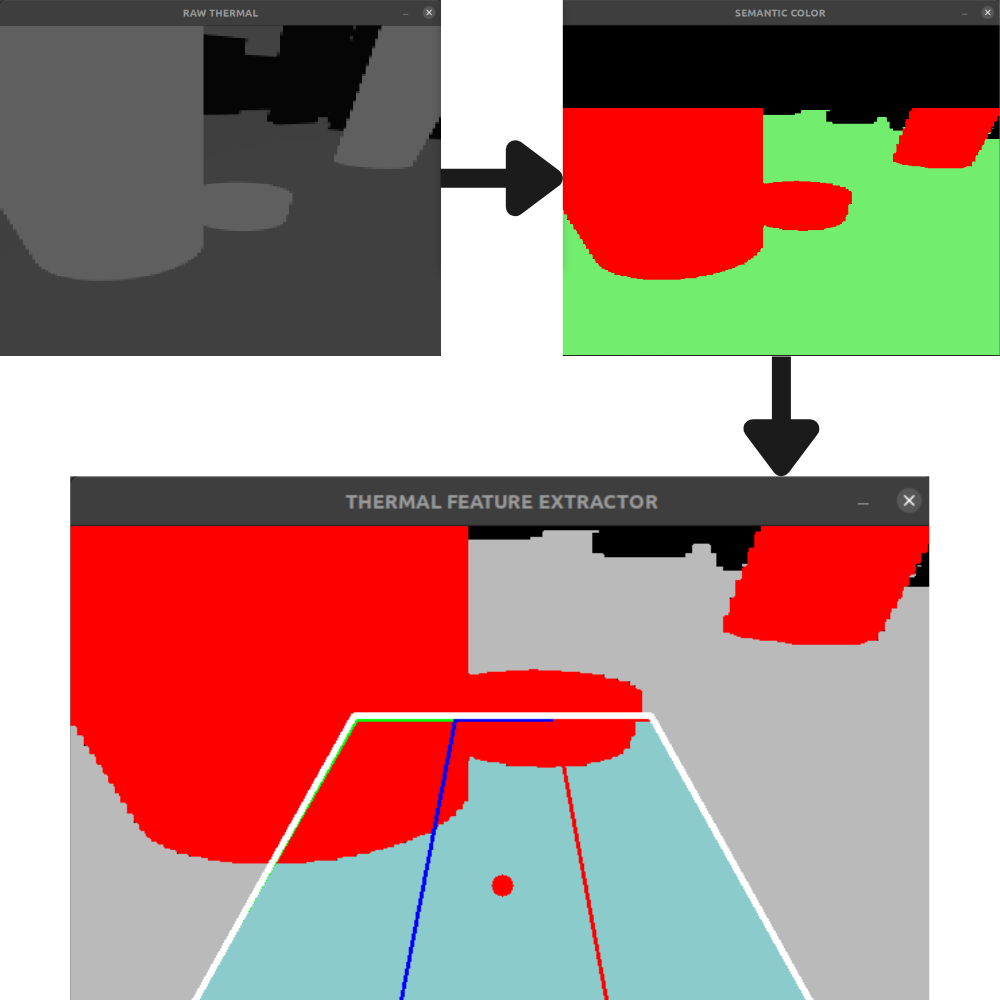
\includegraphics[width=0.5\textwidth]{gambar/3.5_segmentasi_termal.png}
\caption{Contoh hasil segmentasi semantik pada citra termal.}
\label{fig:segmentasi_termal}
\end{figure}

\subsection{Ekstraksi Fitur Traversability}

Setelah proses segmentasi selesai, citra semantik diproses oleh node \texttt{thermal\_feature\-\_extractor.py}. Tahap ini bertujuan mengekstraksi informasi lingkungan yang lebih ringkas dan mudah digunakan oleh sistem navigasi.

Untuk memperoleh informasi yang relevan terhadap pergerakan robot, diterapkan ROI berbentuk trapesium yang merepresentasikan area pengamatan di depan robot. Bentuk trapesium dipilih untuk menyesuaikan perspektif kamera sehingga area yang lebih dekat terhadap robot memiliki bobot pengamatan yang lebih besar.

Berdasarkan ROI tersebut, sistem menghitung skor traversability termal yang merepresentasikan tingkat keterlaluan area di depan robot. Nilai traversability dinyatakan dalam rentang $[0,1]$, dengan nilai mendekati satu menunjukkan area yang relatif bebas obstacle, sedangkan nilai mendekati nol menunjukkan area yang didominasi obstacle termal.

Secara umum, skor traversability dihitung berdasarkan rasio antara area bebas dan area obstacle yang berada di dalam ROI. Nilai ini digunakan sebagai indikator kondisi lingkungan yang nantinya akan digabungkan dengan informasi LiDAR pada proses fusi sensor.

Selain traversability, sistem juga menghitung lebar koridor bebas (\textit{corridor width}) dan posisi tengah koridor (\textit{center path}). Kedua parameter tersebut digunakan untuk menggambarkan distribusi ruang bebas yang tersedia di depan robot.

\subsection{Analisis Zona Navigasi}

Untuk memperoleh informasi spasial yang lebih rinci, area ROI dibagi menjadi tiga zona navigasi, yaitu zona kiri, zona tengah, dan zona kanan. Pembagian ini memungkinkan sistem mengidentifikasi distribusi obstacle secara lateral tanpa harus melakukan analisis citra secara penuh pada setiap siklus pemrosesan.

Pada masing-masing zona dihitung rasio area bebas terhadap total area zona. Nilai rasio tersebut digunakan untuk menunjukkan tingkat keterlaluan setiap sisi jalur navigasi.

Sebagai contoh, apabila nilai zona kiri lebih rendah dibandingkan zona kanan, maka dapat diinterpretasikan bahwa obstacle lebih dominan berada pada sisi kiri robot. Informasi ini berguna untuk membantu sistem menentukan arah penghindaran obstacle yang lebih aman (\cite{Sevastopoulos2022}).

\subsection{Deteksi Area Blind-Spot}

Selain digunakan untuk menghitung traversability, citra termal juga dimanfaatkan untuk mengidentifikasi obstacle yang tidak terdeteksi oleh LiDAR akibat keterbatasan bidang pindai horizontal. Obstacle yang berada pada area blind-spot akan tetap muncul pada citra termal selama memiliki perbedaan temperatur yang cukup terhadap lingkungan sekitarnya.

Untuk tujuan tersebut, node \texttt{semantic\_thermal.py} menghasilkan masker obstacle termal yang dipublikasikan melalui topik:

\begin{center}
\texttt{/thermal\_obstacle\_mask}
\end{center}

Masker ini berisi representasi biner obstacle termal yang telah dipisahkan dari area lantai dan objek latar belakang. Informasi tersebut menjadi dasar untuk membangun representasi obstacle blind-spot pada tahap berikutnya.

Pada tahap ini, informasi termal masih berada dalam domain citra dan belum digunakan secara langsung oleh sistem navigasi. Integrasi dengan data LiDAR dilakukan melalui proses pembentukan \textit{Virtual LaserScan} dan fusi traversability yang akan dijelaskan pada Subbab~\ref{sec:fusi_traversability}.

\section{Fusi Sensor dan Estimasi Traversability}
\label{sec:fusi_traversability}
Setelah informasi geometris dari LiDAR dan informasi termal dari kamera diperoleh, tahap berikutnya adalah mengintegrasikan kedua sumber data tersebut ke dalam representasi yang dapat digunakan oleh sistem navigasi. Integrasi dilakukan melalui dua mekanisme utama. Pertama, obstacle termal yang berada pada area \textit{blind-spot} LiDAR diproyeksikan menjadi \textit{Virtual LaserScan} sehingga dapat diproses oleh ROS Navigation Stack sebagaimana data LiDAR konvensional. Kedua, informasi traversability yang dihasilkan masing-masing sensor digabungkan untuk menghasilkan nilai traversability efektif yang digunakan sebagai masukan bagi pengendali fuzzy.

Pendekatan ini memungkinkan sistem memanfaatkan keunggulan masing-masing sensor secara komplementer. LiDAR menyediakan informasi geometris dengan akurasi tinggi, sedangkan kamera termal mampu mendeteksi obstacle yang tidak teramati oleh bidang pindai LiDAR (\cite{Choi2023,Schichler2025}).

\subsection{Pembentukan Virtual LaserScan dari Kamera Termal}
\label{sec:virtual_laserscan}

Informasi obstacle yang diperoleh dari topik \texttt{/thermal\_obstacle\_mask} tidak dapat digunakan secara langsung oleh ROS Navigation Stack karena masih berada dalam domain citra. Oleh karena itu, penelitian ini membentuk representasi \textit{Virtual LaserScan} yang memiliki format identik dengan keluaran sensor LiDAR.

Proses ini dilakukan oleh node \texttt{thermal\_blindspot\_to\_scan.py}. Node tersebut mene\-rima citra biner obstacle termal beresolusi $640 \times 480$ piksel dengan frekuensi 10 Hz, kemudian menghasilkan topik \texttt{/thermal\_blindspot\_scan} dalam format \texttt{sensor\_msgs/LaserScan}. Dengan pendekatan ini, obstacle termal dapat diproses oleh \textit{costmap} dan APFPlanner tanpa memerlukan modifikasi pada struktur ROS Navigation Stack.

Virtual scan dibentuk menggunakan 61 \textit{beam} yang tersebar pada rentang sudut

\begin{equation}
\theta \in [-0.70,\;0.70]\;\text{rad}
\end{equation}

atau sekitar $\pm 40^\circ$ terhadap arah depan robot. Rentang ini dipilih karena area tersebut merupakan zona yang paling relevan terhadap proses penghindaran obstacle pada navigasi lokal.

\subsection{Proyeksi Obstacle Blind-Spot ke Koordinat Robot}

Sebelum dilakukan proyeksi, masker obstacle termal terlebih dahulu diproses menggunakan operasi morfologi untuk mengurangi noise dan memperbaiki kontinuitas area obstacle. Operasi \textit{opening} digunakan untuk menghilangkan blob kecil yang tidak relevan, sedangkan \textit{closing} digunakan untuk menutup celah pada area obstacle.

Selanjutnya diterapkan pembatasan \textit{region of interest} (ROI) pada 55\% bagian bawah citra. Langkah ini dilakukan karena area tersebut merepresentasikan ruang yang berada dekat dengan robot dan paling berpotensi menyebabkan kolisi. Struktur panas yang berada jauh dari robot tidak dipertimbangkan pada tahap ini karena tidak berkontribusi langsung terhadap keputusan navigasi (\cite{Kibii2022}).

Setiap blob obstacle yang lolos proses seleksi kemudian diproyeksikan ke koordinat polar robot. Posisi vertikal piksel digunakan untuk mengestimasi jarak obstacle terhadap robot, sedangkan posisi horizontal digunakan untuk menentukan arah obstacle relatif terhadap sumbu depan robot.

Jarak estimasi dihitung menggunakan persamaan

\begin{equation}
r = r_{far} + (r_{near}-r_{far})v
\label{eq:range_projection}
\end{equation}

dengan

\begin{equation}
v=\frac{p_y-y_{top}}{h-y_{top}}
\end{equation}

di mana:

\begin{itemize}
\item $r$ adalah estimasi jarak obstacle,
\item $r_{near}$ adalah jarak minimum yang diasosiasikan dengan bagian bawah citra,
\item $r_{far}$ adalah jarak maksimum yang diasosiasikan dengan bagian atas ROI,
\item $p_y$ adalah koordinat vertikal piksel,
\item $h$ adalah tinggi citra.
\end{itemize}

Sementara itu, sudut obstacle dihitung menggunakan

\begin{equation}
u=\frac{p_x-w/2}{w/2}
\end{equation}

\begin{equation}
\theta=-u\alpha_{fov}
\label{eq:angle_projection}
\end{equation}

dengan:

\begin{itemize}
\item $p_x$ adalah koordinat horizontal piksel,
\item $w$ adalah lebar citra,
\item $\alpha_{fov}$ adalah setengah sudut pandang kamera termal.
\end{itemize}

Hasil proyeksi tersebut digunakan untuk mengisi nilai jarak pada \textit{beam} Virtual LaserScan. Dengan demikian, obstacle yang berada pada area blind-spot LiDAR dapat direpresentasikan sebagai obstacle virtual dalam sistem navigasi.

\begin{figure}[H]
\centering
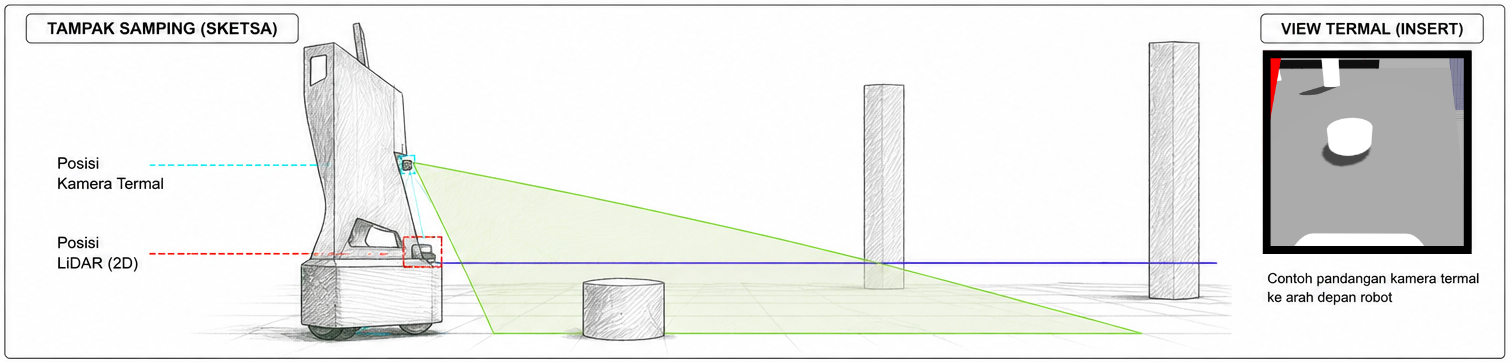
\includegraphics[width=0.85\textwidth]{gambar/3.6_proyeksi_blindspot.png}
\caption{Proses proyeksi obstacle termal ke koordinat polar robot untuk pembentukan Virtual LaserScan.}
\label{fig:proyeksi_blindspot}
\end{figure}

Untuk meningkatkan stabilitas deteksi, sistem menerapkan mekanisme memori temporal. Ketika obstacle termal menghilang sesaat akibat fluktuasi citra atau pergerakan kamera, hasil deteksi terakhir dipertahankan selama interval tertentu sebelum dihapus. Pendekatan ini mencegah terbentuknya perilaku navigasi yang tidak stabil akibat hilangnya obstacle secara tiba-tiba.

\subsection{Traversability Berbasis LiDAR}

Selain digunakan untuk mendeteksi obstacle, data LiDAR juga dimanfaatkan untuk meng\-estimasi tingkat keterlaluan lingkungan di sekitar robot. Konsep traversability digunakan untuk menggambarkan seberapa aman suatu area untuk dilalui berdasarkan ruang bebas yang tersedia (\cite{Sevastopoulos2022}).

Pada penelitian ini, traversability LiDAR dihitung berdasarkan lebar koridor bebas yang tersedia di sekitar arah pergerakan robot. Jarak lateral terhadap obstacle pada sisi kiri dan kanan diperoleh melalui proyeksi komponen jarak LiDAR terhadap sumbu lateral robot.

\begin{equation}
d_{lat}=r_i\sin|\varphi_i|
\label{eq:lateral_distance}
\end{equation}

dengan:

\begin{itemize}
\item $r_i$ adalah jarak LiDAR pada sudut $\varphi_i$,
\item $d_{lat}$ adalah komponen jarak lateral terhadap obstacle.
\end{itemize}

Lebar koridor bebas dihitung sebagai

\begin{equation}
w_{corridor}=d_{left}+d_{right}
\label{eq:corridor_width}
\end{equation}

Nilai tersebut kemudian dinormalisasi menjadi skor traversability LiDAR

\begin{equation}
\tau_{LiDAR}
=
\mathrm{clip}
\left(
\frac{w_{corridor}-w_{robot}}
{w_{ref}},
0,
1
\right)
\label{eq:trav_lidar}
\end{equation}

dengan:

\begin{itemize}
\item $w_{robot}$ adalah lebar robot,
\item $w_{ref}$ adalah lebar koridor referensi.
\end{itemize}

Semakin besar ruang bebas yang tersedia, semakin tinggi nilai traversability yang diperoleh.

\subsection{Fusi Traversability LiDAR--Termal}

Skor traversability yang dihasilkan LiDAR dan kamera termal memiliki karakteristik yang berbeda. Traversability LiDAR menggambarkan kondisi geometris lingkungan, sedangkan traversability termal merepresentasikan keberadaan obstacle berdasarkan informasi panas.

Sebelum dilakukan fusi, nilai traversability termal terlebih dahulu diproses menggunakan \textit{low-pass filter} asimetris. Filter ini dirancang agar sistem dapat merespons kemunculan obstacle secara cepat, namun tetap menghindari perubahan keputusan yang terlalu agresif ketika obstacle menghilang.

Koefisien filter didefinisikan sebagai

\begin{equation}
\alpha=
\begin{cases}
0.50, & \tau_{thermal}<\hat{\tau}_{thermal}\\
0.20, & \tau_{thermal}\geq\hat{\tau}_{thermal}
\end{cases}
\label{eq:lpf_alpha}
\end{equation}

dan pembaruan nilai traversability termal terfilter diberikan oleh

\begin{equation}
\hat{\tau}_{thermal}
=
(1-\alpha)\hat{\tau}_{thermal}
+
\alpha\tau_{thermal}
\label{eq:lpf_update}
\end{equation}

dengan:

\begin{itemize}
\item $\tau_{thermal}$ adalah traversability termal saat ini,
\item $\hat{\tau}_{thermal}$ adalah traversability termal hasil penyaringan.
\end{itemize}

Setelah proses penyaringan selesai, nilai traversability efektif dihitung menggunakan operator minimum

\begin{equation}
\tau_{eff}
=
\min
\left(
\tau_{LiDAR},
\hat{\tau}_{thermal}
\right)
\label{eq:trav_eff}
\end{equation}

Pendekatan ini menerapkan prinsip \textit{safety-first fusion}, yaitu sistem selalu menggunakan kondisi yang paling konservatif dari kedua sensor (\cite{Haider2022,Schichler2025}). Dengan demikian, apabila salah satu sensor mendeteksi kondisi yang tidak aman, nilai traversa\-bility efektif akan menurun sehingga robot dapat merespons lingkungan secara lebih hati-hati.

Nilai traversability efektif $\tau_{eff}$ bersama jarak obstacle terdekat $d_{obs}$ selanjutnya digunakan sebagai masukan pada pengendali fuzzy Mamdani yang akan dijelaskan pada subbab berikutnya.

\section{Fuzzy-Adaptive Artificial Potential Field}
\label{sec:fuzzy_Aapf}
Pada konfigurasi \textit{baseline} (S1--S4), APFPlanner menggunakan parameter navigasi yang bersifat tetap untuk menentukan kecepatan pergerakan robot dan kekuatan gaya tolak terhadap obstacle. Pendekatan tersebut relatif sederhana dan memiliki kompleksitas komputasi yang rendah, namun kurang mampu beradaptasi terhadap perubahan kondisi lingkungan yang terjadi secara dinamis. Ketika robot memasuki area dengan obstacle yang rapat atau traversability lingkungan menurun, penggunaan parameter tetap dapat menghasilkan perilaku navigasi yang terlalu agresif maupun terlalu konservatif.

Untuk mengatasi keterbatasan tersebut, penelitian ini mengintegrasikan logika fuzzy Mamdani sebagai mekanisme adaptasi parameter navigasi. Berbeda dengan pendekatan yang menggunakan fuzzy sebagai pengendali utama robot, sistem fuzzy pada penelitian ini berperan sebagai lapisan adaptif (\textit{adaptive layer}) yang memodifikasi parameter APF berdasarkan kondisi lingkungan yang diamati sensor. Pendekatan serupa telah banyak digunakan pada sistem navigasi robot bergerak karena mampu meningkatkan fleksibilitas pengambilan keputusan tanpa menambah kompleksitas komputasi secara signifikan (\cite{Haider2022,Benaicha2026}).

Masukan sistem fuzzy terdiri atas jarak obstacle terdekat ($d_{obs}$) yang diperoleh dari data LiDAR dan nilai traversability efektif ($\tau_{eff}$) hasil fusi sensor. Berdasarkan kedua informasi tersebut, sistem menghasilkan dua parameter adaptif, yaitu \textit{speed scale} ($S$) dan \textit{repulsive gain} ($G$), yang selanjutnya digunakan untuk menyesuaikan perilaku APFPlanner secara \textit{real-time}.

\subsection{Variabel Input dan Output}

Variabel masukan pertama adalah jarak obstacle terdekat ($d_{obs}$) yang diperoleh dari hasil pemrosesan LiDAR sebagaimana dijelaskan pada Subbab~\ref{sec:pemrosesan_lidar}. Variabel ini digunakan untuk merepresentasikan tingkat kedekatan robot terhadap obstacle yang berada di sekitarnya.

Variabel masukan kedua adalah traversability efektif ($\tau_{eff}$) yang diperoleh melalui meka\-nisme fusi sensor pada Subbab~\ref{sec:fusi_traversability}. Nilai tersebut menggambarkan tingkat keamanan area yang berada di depan robot berdasarkan informasi geometris dan termal.

Sementara itu, sistem fuzzy menghasilkan dua variabel keluaran, yaitu:

\begin{enumerate}
\item \textit{Speed Scale} ($S$), yang digunakan untuk mengatur kecepatan linear robot.
\item \textit{Repulsive Gain} ($G$), yang digunakan untuk mengatur kekuatan gaya tolak obstacle pada APF.
\end{enumerate}

Tabel~\ref{tab:variabel_fuzzy} menunjukkan rentang setiap variabel yang digunakan dalam sistem fuzzy.

\begin{table}[H]
\centering
\caption{Variabel masukan dan keluaran sistem fuzzy}
\label{tab:variabel_fuzzy}
\begin{tabular}{llll}
\toprule
\textbf{Variabel} &
\textbf{Simbol} &
\textbf{Jenis} &
\textbf{Rentang} \\
\midrule
Jarak obstacle &
$d_{obs}$ &
Masukan &
0 -- 6 m \\

Traversability efektif &
$\tau_{eff}$ &
Masukan &
0 -- 1 \\

Speed Scale &
$S$ &
Keluaran &
0 -- 1 \\

Repulsive Gain &
$G$ &
Keluaran &
0 -- 1 \\
\bottomrule
\end{tabular}
\end{table}

% \subsection{Fungsi Keanggotaan}
% \label{sec:fungsi_keanggotaan}

% Setiap variabel fuzzy direpresentasikan menggunakan fungsi keanggotaan berbentuk segitiga dan trapesium. Bentuk fungsi tersebut dipilih karena sederhana, mudah diimplementasikan, serta mampu merepresentasikan perubahan kondisi lingkungan secara bertahap (\cite{Mamdani1974}).

% \subsubsection{Fungsi Keanggotaan Jarak Obstacle}

% Variabel jarak obstacle ($d_{obs}$) dibagi menjadi tiga himpunan linguistik, yaitu:

% \begin{enumerate}
% \item \textit{Near}
% \item \textit{Medium}
% \item \textit{Far}
% \end{enumerate}

% Fungsi keanggotaan yang digunakan ditunjukkan pada Gambar~\ref{fig:mf_jarak}.

% \begin{figure}[H]
% \centering
% 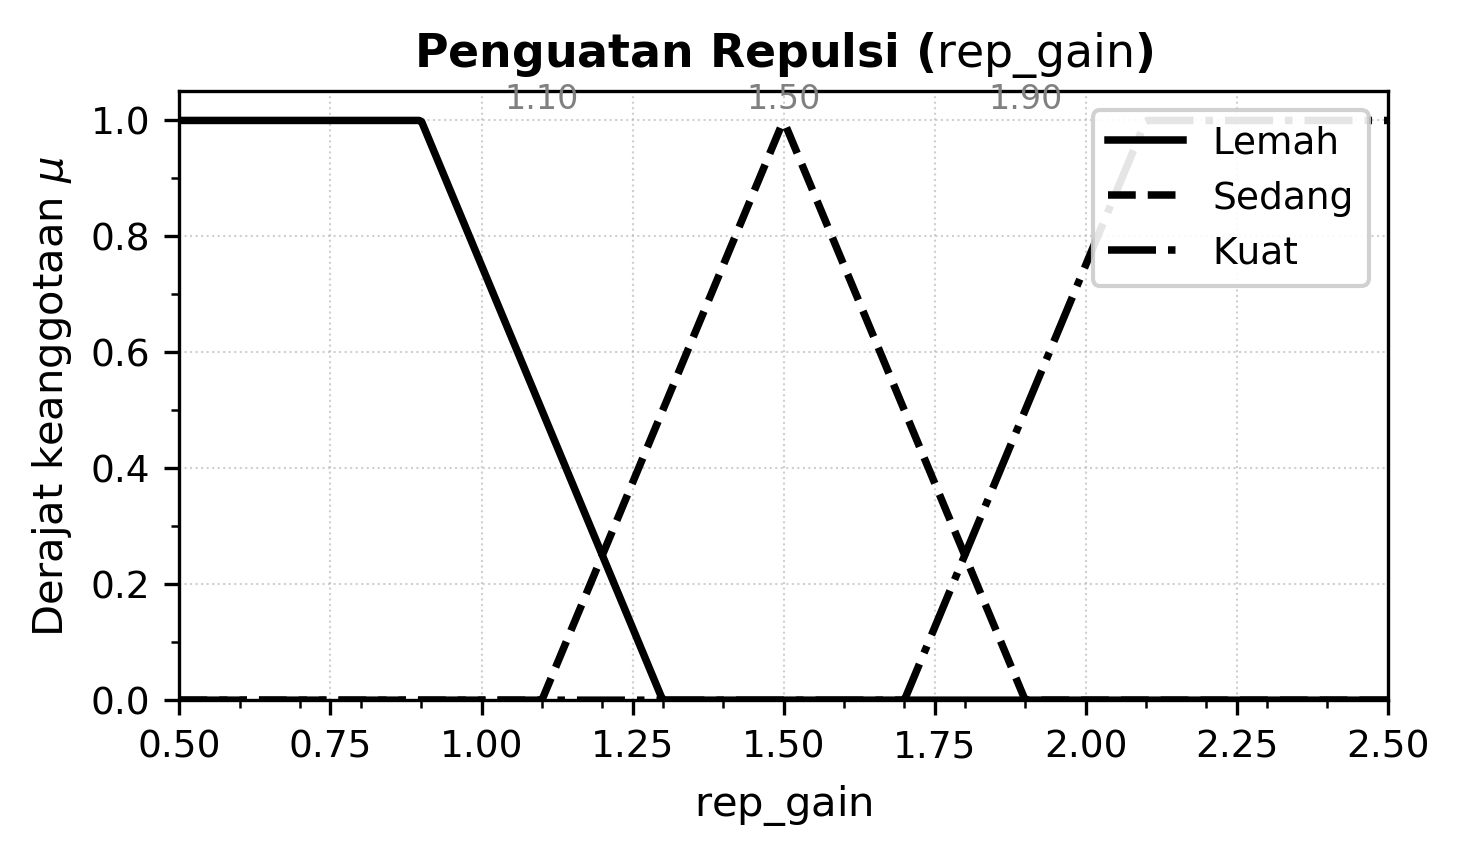
\includegraphics[width=0.8\textwidth]{gambar/3.7_fig_mf_gain.png}
% \caption{Fungsi keanggotaan variabel jarak obstacle.}
% \label{fig:mf_jarak}
% \end{figure}

% \subsubsection{Fungsi Keanggotaan Traversability}

% Variabel traversability efektif ($\tau_{eff}$) dibagi menjadi tiga himpunan linguistik, yaitu:

% \begin{enumerate}
% \item \textit{Low}
% \item \textit{Medium}
% \item \textit{High}
% \end{enumerate}

% Fungsi keanggotaan traversability ditunjukkan pada Gambar~\ref{fig:mf_traversability}.

% \begin{figure}[H]
% \centering
% 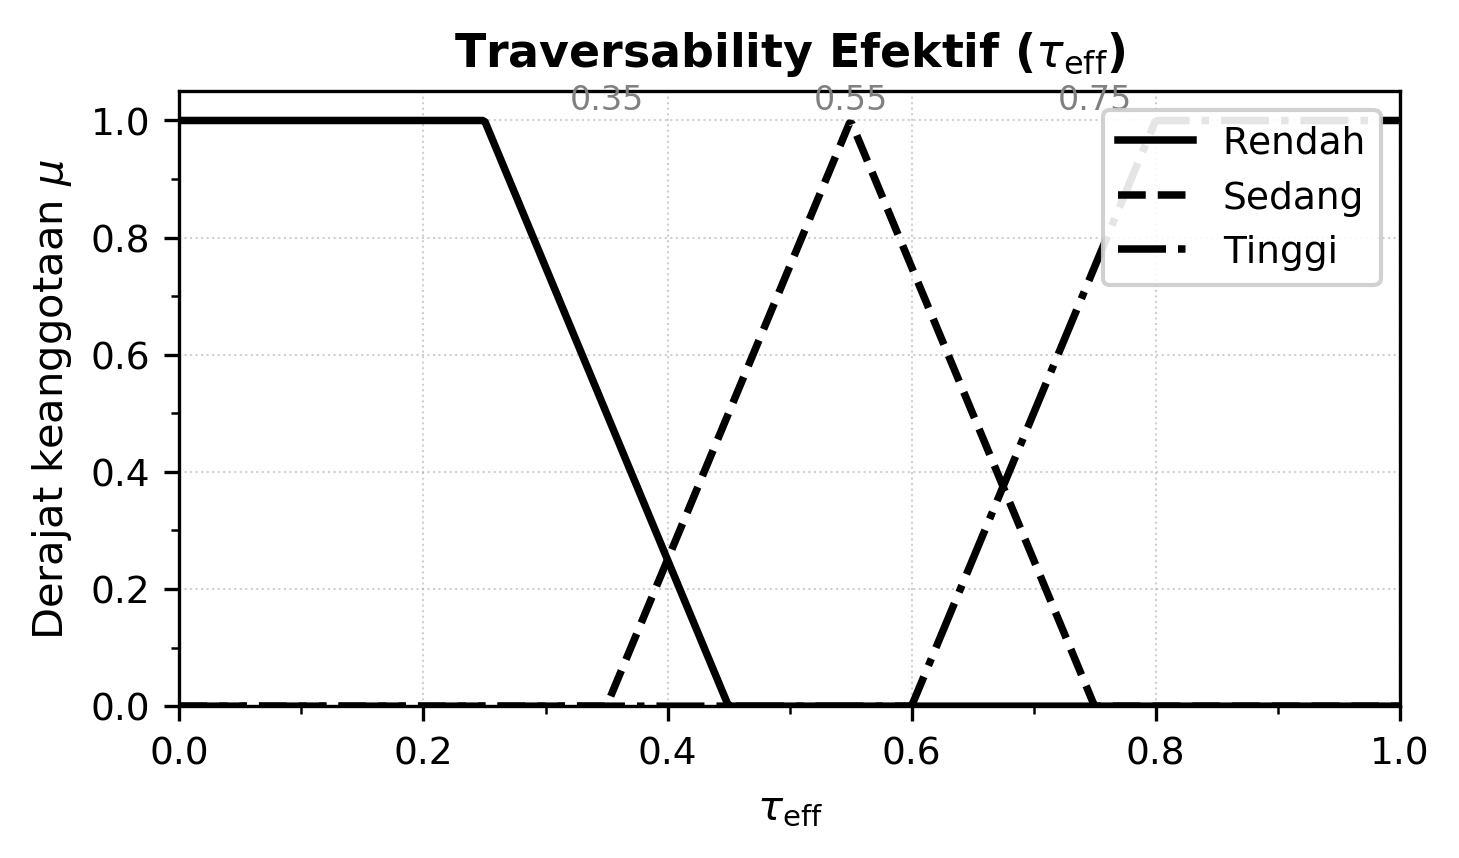
\includegraphics[width=0.8\textwidth]{gambar/3.7_fig_mf_trav.png}
% \caption{Fungsi keanggotaan variabel traversability efektif.}
% \label{fig:mf_traversability}
% \end{figure}

% \subsubsection{Fungsi Keanggotaan Speed Scale}

% Variabel keluaran \textit{Speed Scale} dibagi menjadi tiga himpunan linguistik:

% \begin{enumerate}
% \item \textit{Slow}
% \item \textit{Medium}
% \item \textit{Fast}
% \end{enumerate}

% Fungsi keanggotaan ditunjukkan pada Gambar~\ref{fig:mf_kecepatan}.

% \begin{figure}[H]
% \centering
% 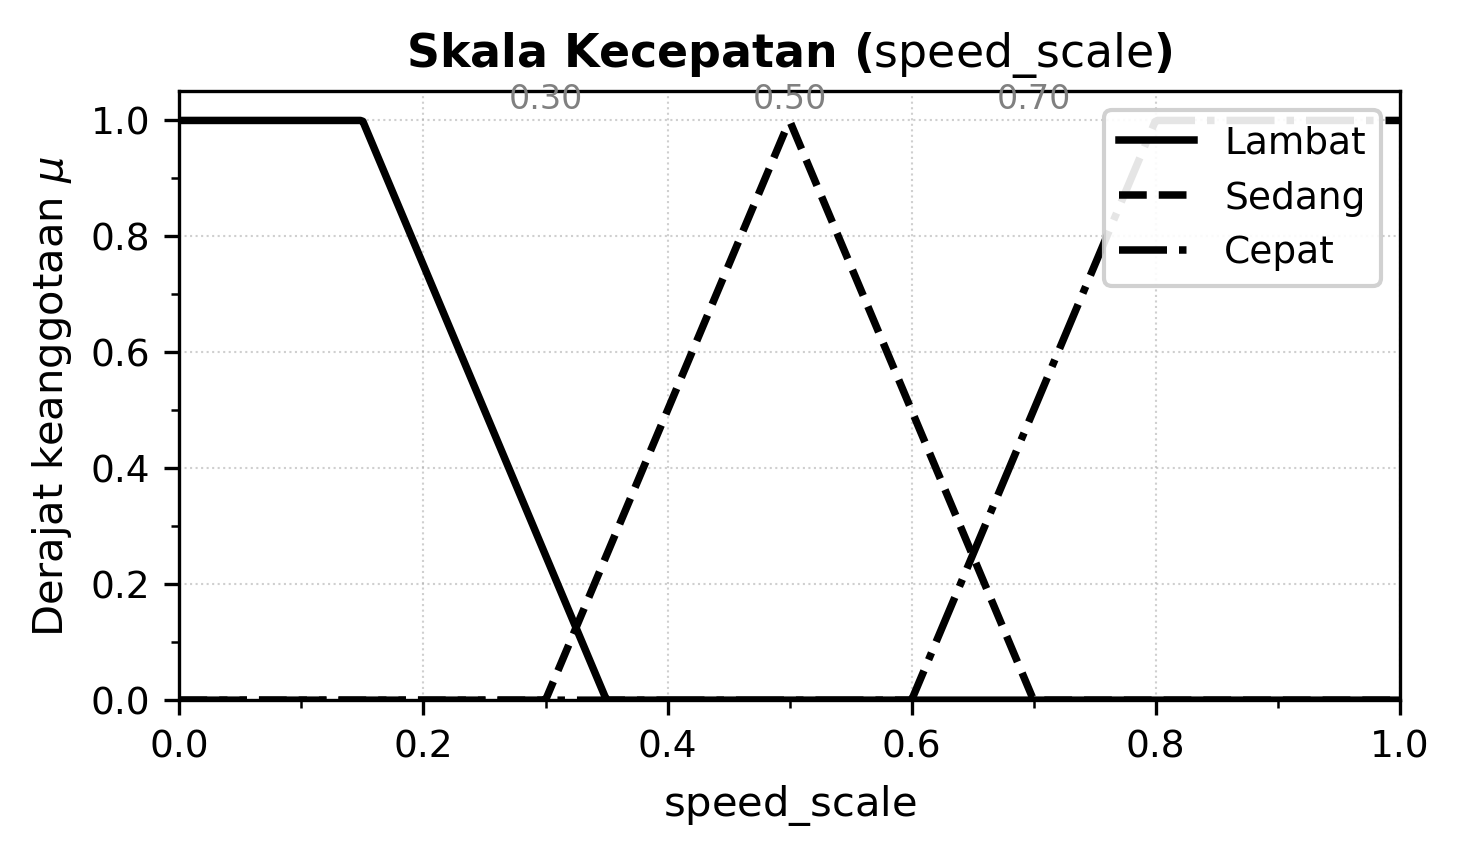
\includegraphics[width=0.8\textwidth]{gambar/3.7_fig_mf_kecepatan.png}
% \caption{Fungsi keanggotaan variabel \textit{Speed Scale}.}
% \label{fig:mf_kecepatan}
% \end{figure}

% \subsubsection{Fungsi Keanggotaan Repulsive Gain}

% Variabel keluaran \textit{Repulsive Gain} dibagi menjadi tiga himpunan linguistik:

% \begin{enumerate}
% \item \textit{Weak}
% \item \textit{Medium}
% \item \textit{Strong}
% \end{enumerate}

% Fungsi keanggotaan ditunjukkan pada Gambar~\ref{fig:mf_gain}.

% \begin{figure}[H]
% \centering
% 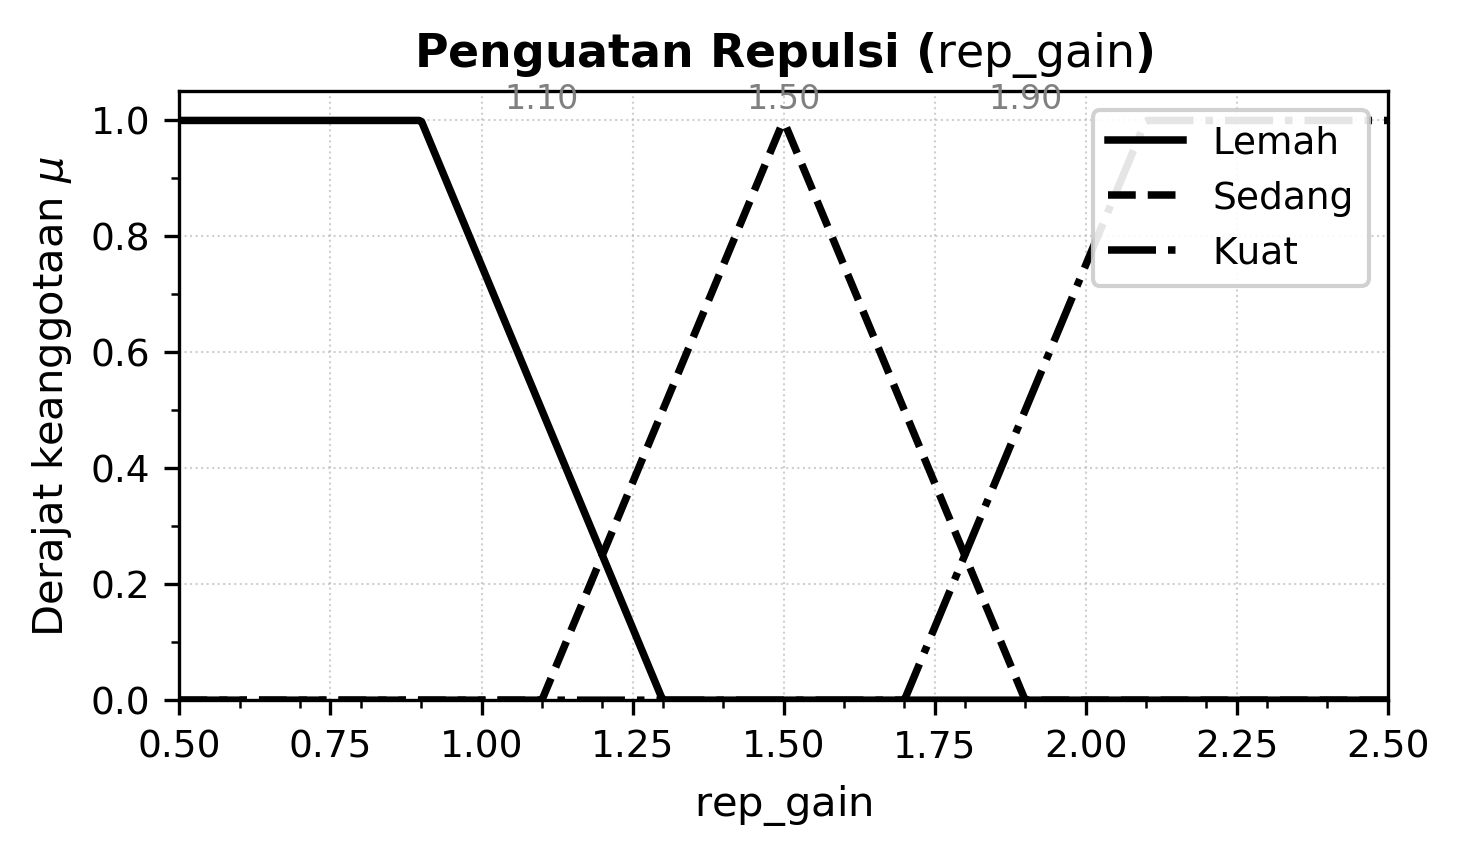
\includegraphics[width=0.8\textwidth]{gambar/3.7_fig_mf_gain.png}
% \caption{Fungsi keanggotaan variabel \textit{Repulsive Gain}.}
% \label{fig:mf_gain}
% \end{figure}

\subsection{Fungsi Keanggotaan}
\label{sec:fuzzy_mf}
% -----------------------------------------------------------------------

Setiap variabel fuzzy didefinisikan menggunakan tiga label linguistik dengan fungsi keanggotaan berbentuk trapesium (\textit{trapmf}) atau segitiga (\textit{trimf}). Bentuk trapesium dipilih untuk label ujung (rendah/lambat/lemah dan tinggi/cepat/kuat) karena memberikan respons jenuh (\textit{saturation}) di area ekstrem, sehingga nilai input yang sangat ekstrem selalu mendapatkan keanggotaan penuh pada label tersebut~\cite{Benaicha2026}. Bentuk segitiga dipilih untuk label tengah karena memberikan transisi yang halus dan simetris.

Fungsi keanggotaan didefinisikan sebagai berikut. Untuk fungsi segitiga:
\begin{equation}
    \mu_\text{trimf}(x;\,a,b,c) =
    \begin{cases}
        0 & x \leq a \\
        \dfrac{x - a}{b - a} & a < x \leq b \\[6pt]
        \dfrac{c - x}{c - b} & b < x \leq c \\
        0 & x > c
    \end{cases}
    \label{eq:trimf}
\end{equation}
dan untuk fungsi trapesium:
\begin{equation}
    \mu_\text{trapmf}(x;\,a,b,c,d) =
    \begin{cases}
        0 & x \leq a \\
        \dfrac{x - a}{b - a} & a < x \leq b \\[4pt]
        1 & b < x \leq c \\[4pt]
        \dfrac{d - x}{d - c} & c < x \leq d \\
        0 & x > d
    \end{cases}
    \label{eq:trapmf}
\end{equation}
Kasus khusus $a = b$ (tepi naik vertikal) atau $c = d$ (tepi turun vertikal) ditangani sebagai nilai langsung 1 atau 0 pada titik tersebut, konsisten dengan implementasi \texttt{skfuzzy.trapmf}.

\subsubsection*{a. Fungsi Keanggotaan Input: Jarak \textit{Obstacle} ($d_\text{obs}$)}

Input jarak didefinisikan dengan tiga label pada domain $[0{,}0,\ 2{,}0]$~m:
\begin{align}
    \mu_\text{dekat}(d)  &= \mu_\text{trapmf}(d;\;0{,}00,\;0{,}00,\;0{,}30,\;0{,}60) \label{eq:mf_dekat} \\
    \mu_\text{sedang}(d) &= \mu_\text{trimf}(d;\;0{,}40,\;0{,}80,\;1{,}20)           \label{eq:mf_sedang_d} \\
    \mu_\text{jauh}(d)   &= \mu_\text{trapmf}(d;\;1{,}00,\;1{,}40,\;2{,}00,\;2{,}00) \label{eq:mf_jauh}
\end{align}
Label \textit{Dekat} memiliki keanggotaan penuh untuk jarak $d \leq 0{,}30$~m dan menurun hingga nol pada $d = 0{,}60$~m. Label \textit{Jauh} mulai naik dari $d = 1{,}00$~m dan mencapai keanggotaan penuh pada $d \geq 1{,}40$~m.

\subsubsection*{b. Fungsi Keanggotaan Input: Traversability ($\tau_\text{eff}$)}

Input traversability didefinisikan dengan tiga label pada domain $[0{,}0,\ 1{,}0]$:
\begin{align}
    \mu_\text{rendah}(\tau) &= \mu_\text{trapmf}(\tau;\;0{,}00,\;0{,}00,\;0{,}25,\;0{,}45) \label{eq:mf_rendah} \\
    \mu_\text{sedang}(\tau) &= \mu_\text{trimf}(\tau;\;0{,}35,\;0{,}55,\;0{,}75)           \label{eq:mf_sedang_t} \\
    \mu_\text{tinggi}(\tau) &= \mu_\text{trapmf}(\tau;\;0{,}60,\;0{,}80,\;1{,}00,\;1{,}00) \label{eq:mf_tinggi}
\end{align}
Label \textit{Rendah} mencakup kondisi ketika jalur banyak terhalang \textit{obstacle} termal atau koridor sempit. Label \textit{Tinggi} mencakup kondisi jalur bebas dan koridor lebar.

\subsubsection*{c. Fungsi Keanggotaan Output: Skala Kecepatan}

Output kecepatan didefinisikan dengan tiga label pada domain $[0{,}0,\ 1{,}0]$:
\begin{align}
    \mu_\text{lambat}(s) &= \mu_\text{trapmf}(s;\;0{,}00,\;0{,}00,\;0{,}15,\;0{,}35) \label{eq:mf_lambat} \\
    \mu_\text{sedang}(s) &= \mu_\text{trimf}(s;\;0{,}30,\;0{,}50,\;0{,}70)           \label{eq:mf_sedang_s} \\
    \mu_\text{cepat}(s)  &= \mu_\text{trapmf}(s;\;0{,}60,\;0{,}80,\;1{,}00,\;1{,}00) \label{eq:mf_cepat}
\end{align}

\subsubsection*{d. Fungsi Keanggotaan Output: Penguatan Repulsi}

Output penguatan repulsi didefinisikan dengan tiga label pada domain $[0{,}5,\ 2{,}5]$:
\begin{align}
    \mu_\text{lemah}(g)  &= \mu_\text{trapmf}(g;\;0{,}5,\;0{,}5,\;0{,}9,\;1{,}3) \label{eq:mf_lemah} \\
    \mu_\text{sedang}(g) &= \mu_\text{trimf}(g;\;1{,}1,\;1{,}5,\;1{,}9)           \label{eq:mf_sedang_g} \\
    \mu_\text{kuat}(g)   &= \mu_\text{trapmf}(g;\;1{,}7,\;2{,}1,\;2{,}5,\;2{,}5) \label{eq:mf_kuat}
\end{align}

Tabel~\ref{tab:fuzzy_mf} merangkum seluruh parameter fungsi keanggotaan dan Gambar~\ref{fig:mf_jarak}--\ref{fig:mf_gain} menam\-pilkan kurva masing-masing variabel.

\begin{table}[H]
\centering
\caption{Parameter fungsi keanggotaan seluruh variabel fuzzy.}
\label{tab:fuzzy_mf}
\begin{tabular}{llllp{4.5cm}}
\toprule
\textbf{Variabel} & \textbf{Label} & \textbf{Tipe} & \textbf{Parameter} & \textbf{Domain} \\
\midrule
\multirow{3}{*}{Jarak ($d$, m)}
  & Dekat  & trapmf & $(0{,}00,\ 0{,}00,\ 0{,}30,\ 0{,}60)$ & $[0{,}0,\ 2{,}0]$~m \\
  & Sedang & trimf  & $(0{,}40,\ 0{,}80,\ 1{,}20)$ & \\
  & Jauh   & trapmf & $(1{,}00,\ 1{,}40,\ 2{,}00,\ 2{,}00)$ & \\
\midrule
\multirow{3}{*}{Traversability ($\tau$)}
  & Rendah & trapmf & $(0{,}00,\ 0{,}00,\ 0{,}25,\ 0{,}45)$ & $[0{,}0,\ 1{,}0]$ \\
  & Sedang & trimf  & $(0{,}35,\ 0{,}55,\ 0{,}75)$ & \\
  & Tinggi & trapmf & $(0{,}60,\ 0{,}80,\ 1{,}00,\ 1{,}00)$ & \\
\midrule
\multirow{3}{*}{Kecepatan ($s$)}
  & Lambat & trapmf & $(0{,}00,\ 0{,}00,\ 0{,}15,\ 0{,}35)$ & $[0{,}0,\ 1{,}0]$ \\
  & Sedang & trimf  & $(0{,}30,\ 0{,}50,\ 0{,}70)$ & \\
  & Cepat  & trapmf & $(0{,}60,\ 0{,}80,\ 1{,}00,\ 1{,}00)$ & \\
\midrule
\multirow{3}{*}{Gain repulsi ($g$)}
  & Lemah  & trapmf & $(0{,}50,\ 0{,}50,\ 0{,}90,\ 1{,}30)$ & $[0{,}5,\ 2{,}5]$ \\
  & Sedang & trimf  & $(1{,}10,\ 1{,}50,\ 1{,}90)$ & \\
  & Kuat   & trapmf & $(1{,}70,\ 2{,}10,\ 2{,}50,\ 2{,}50)$ & \\
\bottomrule
\end{tabular}
\end{table}

\begin{figure}[H]
    \centering
    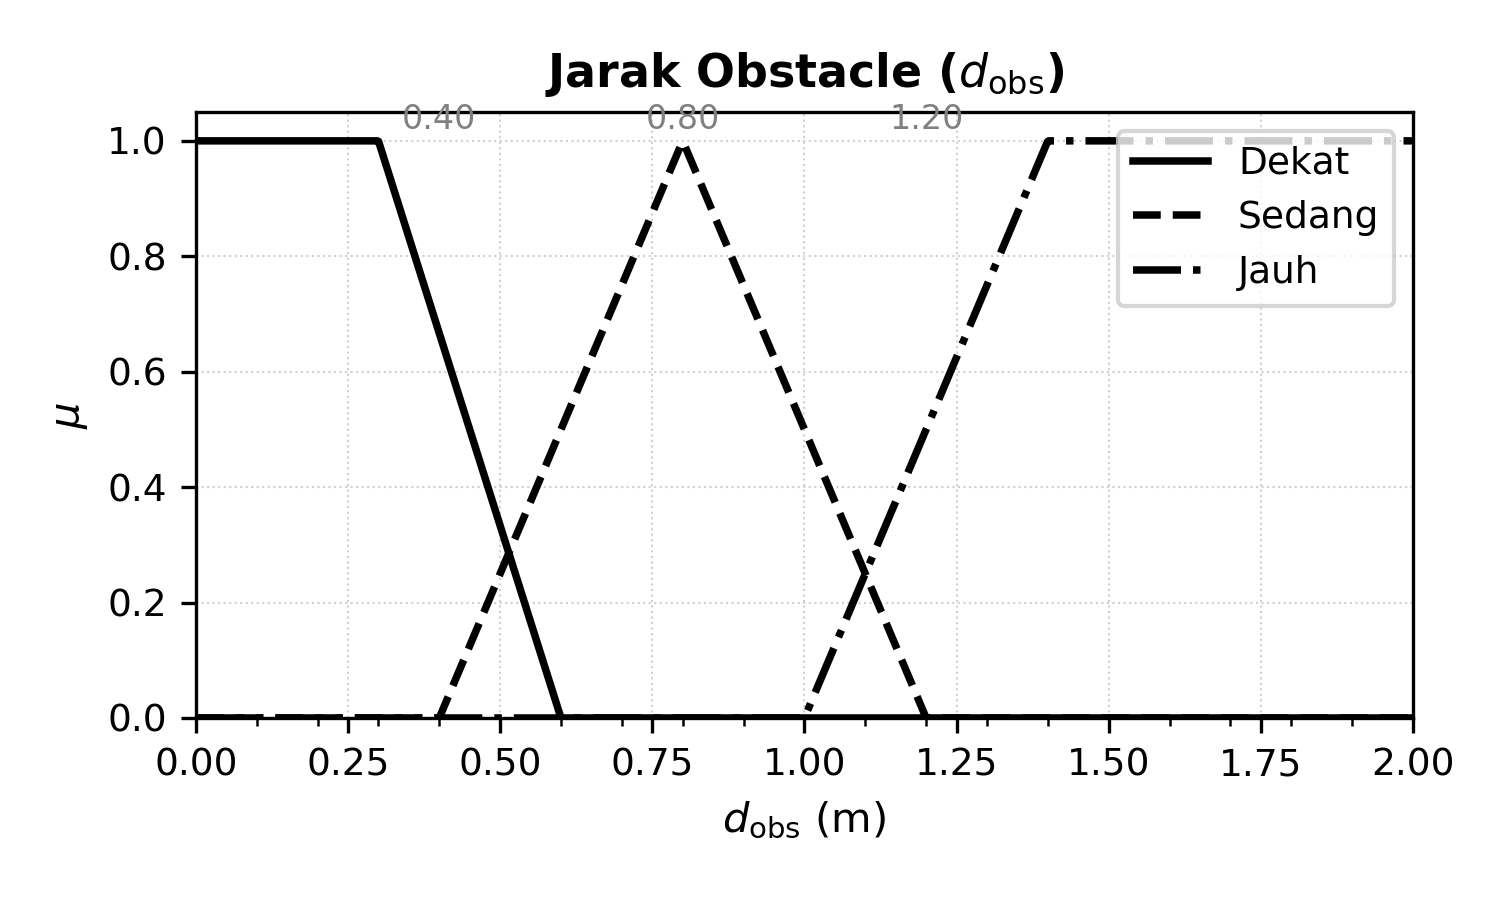
\includegraphics[width=0.48\textwidth]{gambar/3.7_fig_mf_jarak.png} %gambar/fig_mf_jarak
    \hfill
    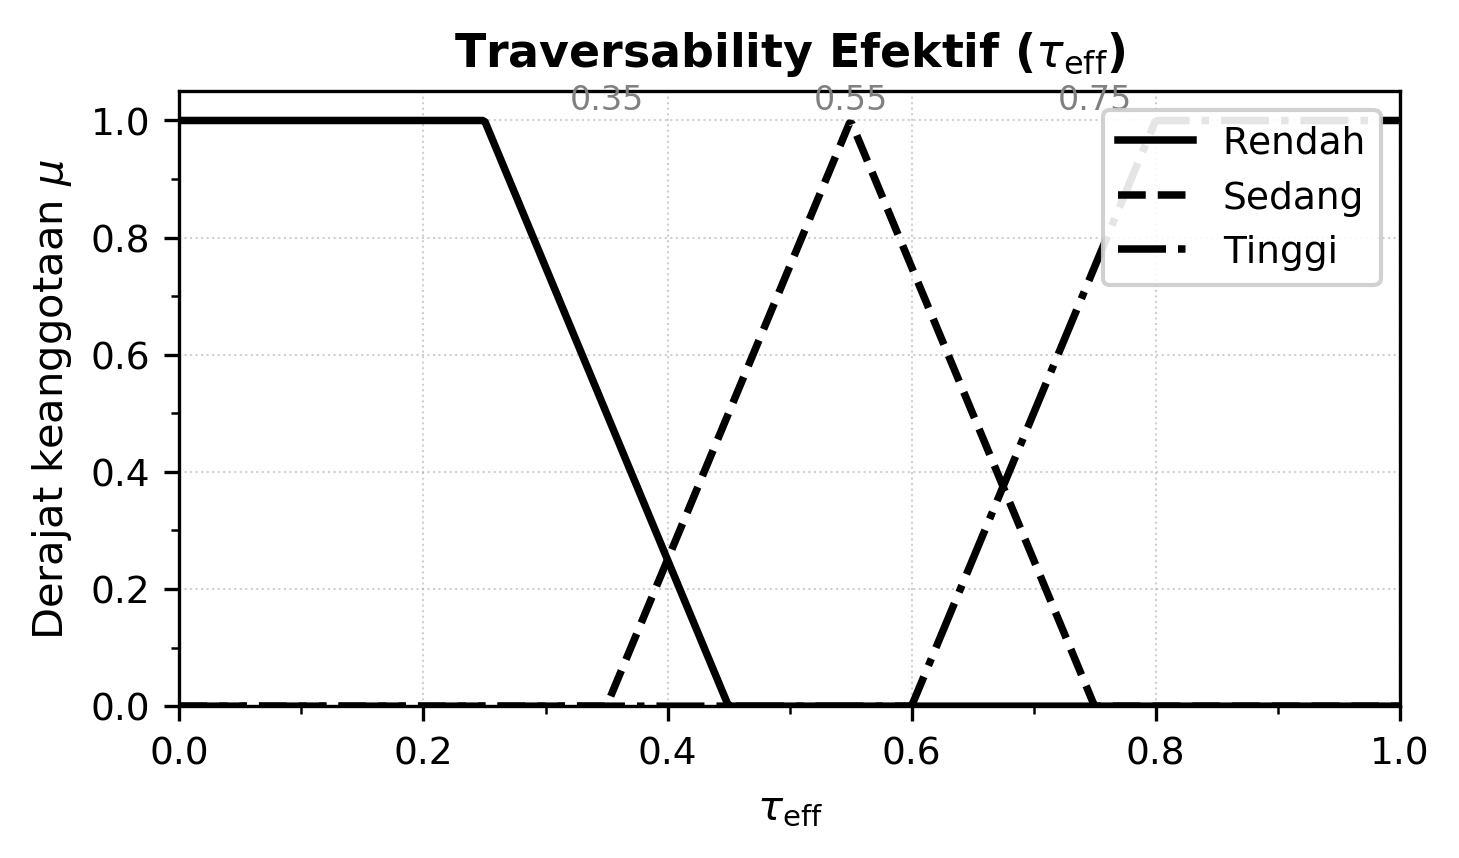
\includegraphics[width=0.48\textwidth]{gambar/3.7_fig_mf_trav.png} %gambar/fig_mf_trav
    \caption{Fungsi keanggotaan variabel input. Kiri: jarak \textit{obstacle} ($d_\text{obs}$, domain $[0, 2]$~m). Kanan: \textit{traversability} efektif ($\tau_\text{eff}$, domain $[0, 1]$).}
    \label{fig:mf_jarak}
\end{figure}

\begin{figure}[H]
    \centering
    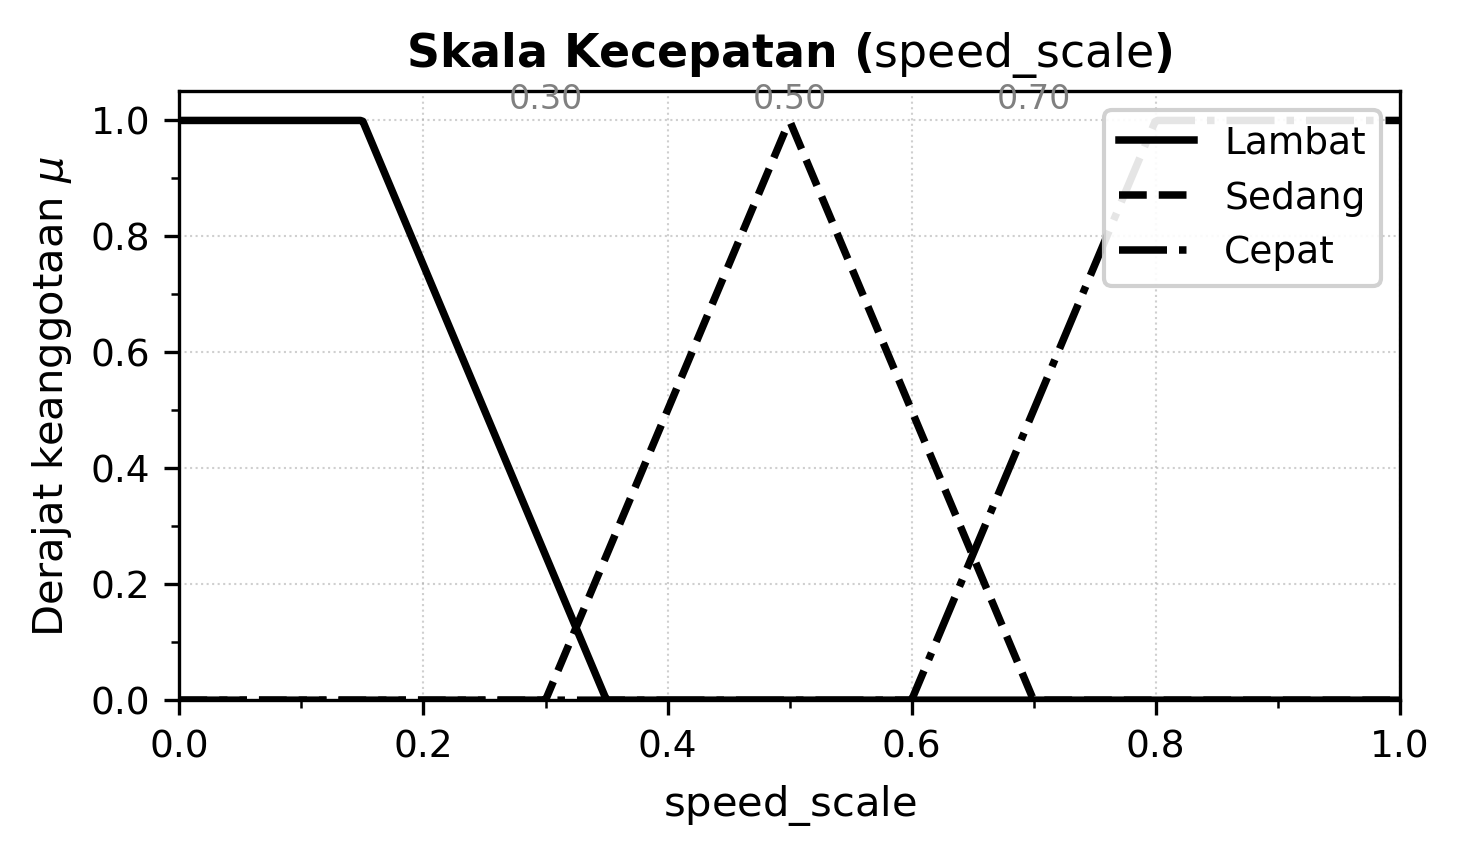
\includegraphics[width=0.48\textwidth]{gambar/3.7_fig_mf_kecepatan.png} %gambar/fig_mf_kecepatan
    \hfill
    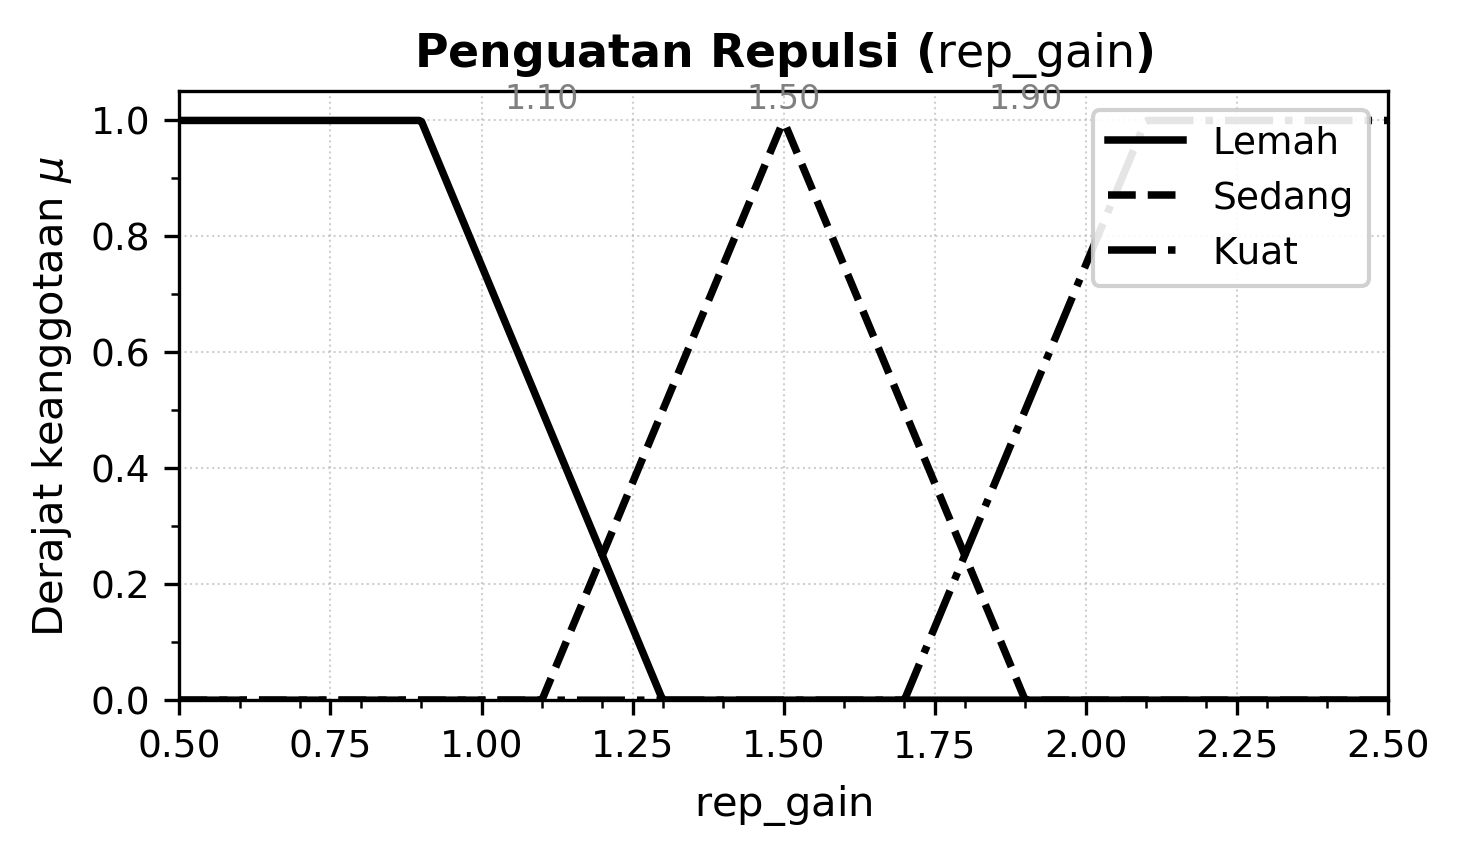
\includegraphics[width=0.48\textwidth]{gambar/3.7_fig_mf_gain.png} %gambar/fig_mf_gain
    \caption{Fungsi keanggotaan variabel output. Kiri: skala kecepatan (\textit{speed\_scale}, domain $[0, 1]$). Kanan: penguatan repulsi (\textit{rep\_gain}, domain $[0{,}5, 2{,}5]$).}
    \label{fig:mf_gain}
\end{figure}

\subsection{Basis Aturan Fuzzy}
\label{sec:basis_aturan}

Hubungan antara variabel masukan dan keluaran direpresentasikan menggunakan sembilan aturan fuzzy Mamdani. Aturan tersebut dirancang berdasarkan prinsip dasar navigasi robot bergerak, yaitu memperlambat robot dan memperbesar gaya tolak ketika obstacle semakin dekat atau traversability lingkungan menurun.

Tabel~\ref{tab:rule_base} menunjukkan basis aturan yang digunakan.

\begin{table}[H]
\centering
\caption{Basis aturan fuzzy Mamdani}
\label{tab:rule_base}
\begin{tabular}{cccc}
\toprule
\multirow{2}{*}{$d_{obs}$}
&
\multicolumn{3}{c}{$\tau_{eff}$}
\\
\cmidrule(lr){2-4}
&
Low &
Medium &
High
\\
\midrule
Near
&
Slow, Strong
&
Slow, Strong
&
Medium, Strong
\\

Medium
&
Slow, Strong
&
Medium, Medium
&
Fast, Medium
\\

Far
&
Medium, Medium
&
Fast, Weak
&
Fast, Weak
\\
\bottomrule
\end{tabular}
\end{table}

Aturan fuzzy yang digunakan dapat dituliskan sebagai berikut:

\begin{enumerate}
\item IF $d_{obs}$ is Near AND $\tau_{eff}$ is Low THEN Speed is Slow AND Gain is Strong.
\item IF $d_{obs}$ is Near AND $\tau_{eff}$ is Medium THEN Speed is Slow AND Gain is Strong.
\item IF $d_{obs}$ is Near AND $\tau_{eff}$ is High THEN Speed is Medium AND Gain is Strong.
\item IF $d_{obs}$ is Medium AND $\tau_{eff}$ is Low THEN Speed is Slow AND Gain is Strong.
\item IF $d_{obs}$ is Medium AND $\tau_{eff}$ is Medium THEN Speed is Medium AND Gain is Medium.
\item IF $d_{obs}$ is Medium AND $\tau_{eff}$ is High THEN Speed is Fast AND Gain is Medium.
\item IF $d_{obs}$ is Far AND $\tau_{eff}$ is Low THEN Speed is Medium AND Gain is Medium.
\item IF $d_{obs}$ is Far AND $\tau_{eff}$ is Medium THEN Speed is Fast AND Gain is Weak.
\item IF $d_{obs}$ is Far AND $\tau_{eff}$ is High THEN Speed is Fast AND Gain is Weak.
\end{enumerate}

\subsection{Inferensi dan Defuzzifikasi}

Metode inferensi yang digunakan adalah Mamdani dengan operator AND berupa minimum (\textit{minimum operator}). Kekuatan aktivasi aturan ke-$k$ dihitung menggunakan:

\begin{equation}
w_k
=
\min
\left(
\mu_A(d_{obs}),
\mu_B(\tau_{eff})
\right)
\label{eq:fuzzy_rule_strength}
\end{equation}

dengan:

\begin{itemize}
\item $w_k$ adalah kekuatan aktivasi aturan ke-$k$,
\item $\mu_A(d_{obs})$ adalah derajat keanggotaan jarak obstacle,
\item $\mu_B(\tau_{eff})$ adalah derajat keanggotaan traversability.
\end{itemize}

Seluruh keluaran aturan kemudian digabungkan menggunakan operator maksimum:

\begin{equation}
\mu_{agg}(y)
=
\max
\left(
\mu_1(y),
\mu_2(y),
\dots,
\mu_n(y)
\right)
\label{eq:fuzzy_aggregation}
\end{equation}

Tahap terakhir adalah defuzzifikasi menggunakan metode \textit{Center of Gravity} (CoG):

\begin{equation}
y^*
=
\frac
{\int y\,\mu_{agg}(y)\,dy}
{\int \mu_{agg}(y)\,dy}
\label{eq:fuzzy_centroid}
\end{equation}

dengan $y^*$ merupakan nilai crisp keluaran fuzzy.

Melalui proses tersebut diperoleh nilai \textit{Speed Scale} dan \textit{Repulsive Gain} yang digunakan untuk menyesuaikan perilaku navigasi robot.

\subsection{Integrasi Fuzzy dengan APFPlanner}

Nilai \textit{Speed Scale} dan \textit{Repulsive Gain} yang dihasilkan oleh sistem fuzzy digunakan untuk memodifikasi parameter APFPlanner secara \textit{real-time}.

Kecepatan linear robot dihitung menggunakan:

\begin{equation}
v
=
S
\cdot
v_{base}
\label{eq:fuzzy_speed_scale}
\end{equation}

dengan:

\begin{itemize}
\item $v$ adalah kecepatan linear aktual robot,
\item $v_{base}$ adalah kecepatan dasar APF,
\item $S$ adalah keluaran \textit{Speed Scale}.
\end{itemize}

Sementara itu, gaya tolak APF dimodifikasi menggunakan:

\begin{equation}
F_{rep}
=
G
\cdot
F_{rep}^{base}
\label{eq:fuzzy_repulsive_gain}
\end{equation}

dengan:

\begin{itemize}
\item $F_{rep}$ adalah gaya tolak setelah adaptasi,
\item $F_{rep}^{base}$ adalah gaya tolak dasar APF,
\item $G$ adalah keluaran \textit{Repulsive Gain}.
\end{itemize}

Melalui mekanisme tersebut, robot dapat bergerak lebih cepat ketika kondisi lingkungan aman dan secara otomatis memperlambat pergerakan serta meningkatkan kemampuan penghindaran obstacle ketika traversability menurun atau obstacle berada pada jarak yang dekat. Integrasi ini menghasilkan sistem \textit{Fuzzy-Adaptive Artificial Potential Field} yang lebih adaptif dibandingkan APF konvensional dengan parameter tetap.

\section{Skenario dan Prosedur Pengujian}
\label{sec:eksperimen}
Setelah seluruh komponen sistem navigasi diimplementasikan dan diintegrasikan ke dalam lingkungan simulasi, tahap berikutnya adalah melakukan pengujian untuk mengevaluasi pengaruh integrasi kamera termal dan pengendali fuzzy terhadap performa navigasi robot. Pengujian dirancang untuk merepresentasikan berbagai kondisi lingkungan yang umum dijumpai pada navigasi robot bergerak di area dalam ruangan, mulai dari lingkungan tanpa obstacle hingga lingkungan dengan obstacle dinamis.

\subsection{Tujuan Pengujian}

Pengujian dilakukan untuk mengevaluasi kemampuan sistem dalam mendeteksi obstacle pada area blind-spot LiDAR, menghindari obstacle statis maupun dinamis, serta mencapai tujuan navigasi secara aman dan efisien.

Secara khusus, pengujian bertujuan untuk:

\begin{enumerate}
\item Mengevaluasi kemampuan integrasi LiDAR dan kamera termal dalam meningkatkan per\-sepsi lingkungan.
\item Menganalisis pengaruh pengendali fuzzy terhadap perilaku navigasi robot.
\item Membandingkan performa sistem baseline dan sistem fuzzy pada kondisi lingkungan yang identik.
\item Mengukur stabilitas dan keamanan navigasi pada berbagai skenario obstacle.
\end{enumerate}

\subsection{Konfigurasi Skenario Pengujian}

Eksperimen dilakukan menggunakan delapan skenario yang dibagi menjadi dua kelompok, yaitu kelompok baseline dan kelompok fuzzy. Seluruh skenario menggunakan peta, robot, dan konfigurasi sensor yang sama sehingga perbedaan performa yang diamati hanya dipengaruhi oleh mekanisme pengendalian yang digunakan.

Tabel~\ref{tab:skenario_pengujian} menunjukkan konfigurasi skenario yang digunakan.

\begin{table}[H]
\centering
\caption{Skenario pengujian yang digunakan}
\label{tab:skenario_pengujian}
\begin{tabular}{cccc}
\toprule
\textbf{Skenario} &
\textbf{Kelompok} &
\textbf{Kondisi Lingkungan} &
\textbf{Fuzzy} \\
\midrule
S1 & Baseline & Tanpa obstacle & Tidak \\
S2 & Baseline & Satu obstacle manusia & Tidak \\
S3 & Baseline & Multiple obstacle statis & Tidak \\
S4 & Baseline & Multiple obstacle dinamis & Tidak \\
S5 & Fuzzy & Tanpa obstacle & Ya \\
S6 & Fuzzy & Satu obstacle manusia & Ya \\
S7 & Fuzzy & Multiple obstacle statis & Ya \\
S8 & Fuzzy & Multiple obstacle dinamis & Ya \\
\bottomrule
\end{tabular}
\end{table}

\subsubsection*{a. Skenario S1/S5 --- Navigasi Tanpa Obstacle}

Skenario S1 dan S5 menggunakan lingkungan \texttt{S1\_open.world} yang tidak mengandung obstacle aktif selain dinding dan struktur peta statis. Skenario ini berfungsi sebagai \textit{control condition} untuk mengisolasi efek logika fuzzy terhadap pola navigasi robot pada kondisi bebas gangguan. Pada S5, \textit{fuzzy controller} aktif meskipun tidak ada obstacle terdekat, sehingga $d_\text{obs}$ selalu tinggi dan $\tau_\text{eff} \approx 1{,}0$; sesuai basis aturan, robot diizinkan bergerak dengan kecepatan penuh dan gain lemah. Selisih kecepatan dan panjang lintasan antara S1 dan S5 menjadi indikator \textit{overhead} yang ditimbulkan fuzzy pada kondisi normal.

\subsubsection*{b. Skenario S2/S6 --- Satu Obstacle Statis}

Skenario S2 dan S6 menggunakan lingkungan \texttt{S2\_single\_human.world} yang memuat satu \textit{obstacle} manusia statis (silinder $r = 0{,}25$~m, tinggi 3~m, posisi $(2{,}466;\ 1{,}273)$~m) yang dapat dideteksi oleh LiDAR. Skenario ini menguji kemampuan dasar penghindaran \textit{obstacle} konvensional serta efek logika fuzzy terhadap \textit{clearance} pada kondisi \textit{obstacle} tunggal. Tidak terdapat \textit{obstacle} kucing pada skenario ini.

\subsubsection*{c. Skenario S3/S7 --- Obstacle Majemuk Statis dengan Kucing}

Skenario S3 dan S7 merupakan skenario utama yang menguji hipotesis penelitian, yaitu apakah sistem mampu menghindari \textit{obstacle} kucing yang tidak terdeteksi LiDAR. Lingkungan \texttt{S3\_static\_multi.world} memuat tiga \textit{obstacle} statis, yaitu: (a) satu \textit{obstacle} statis standar ($r = 0{,}25$~m), (b) \texttt{obstacle\_cat} ($r = 0{,}18$~m, tinggi $\approx$0,19~m, posisi $(2{,}83;\ 0{,}97)$~m) yang berada di \textit{blind-spot} LiDAR, dan (c) dua \textit{obstacle\_human} statis ($r = 0{,}25$~m, tinggi 3~m). Pasangan S3/S7 memungkinkan perbandingan \textit{clearance} terhadap kucing antara konfigurasi \textit{baseline} dan fuzzy dalam kondisi yang terkontrol.

\subsubsection*{d. Skenario S4/S8 --- Obstacle Majemuk Dinamis dengan Kucing}

Skenario S4 dan S8 menambahkan lapisan kompleksitas dengan menggerakkan kedua \textit{obstacle} manusia secara osilasi mulus menggunakan skrip \texttt{dynamic\_obstacles.py}. Masing-masing \textit{obstacle} manusia bergerak bolak-balik di sepanjang jalur linear: human\_1 menempuh jalur sepanjang $\approx 3{,}07$~m dan human\_2 sepanjang $\approx 3{,}23$~m, keduanya dengan profil kecepatan sinusoidal yang menghasilkan kecepatan puncak masing-masing $\approx 0{,}77$~m/s dan $\approx 0{,}81$~m/s. Gerak osilasi dimodelkan menggunakan fungsi:
\begin{equation}
    s(t) = \frac{1}{2}\bigl(1 - \cos(\omega t)\bigr),
    \quad \omega = 0{,}5~\text{rad/s}
    \label{eq:osilasi_human}
\end{equation}
di mana $s(t) \in [0, 1]$ adalah parameter posisi ternormalisasi di sepanjang jalur masing-masing \textit{obstacle} ($s=0$: titik A, $s=1$: titik B). Fungsi kosinus terbalik ini menghasilkan gerakan yang halus dengan akselerasi dan deselerasi di kedua ujung jalur, sehingga menghindari perubahan kecepatan mendadak yang tidak realistis. Posisi \textit{obstacle} diperbarui melalui layanan \texttt{/gazebo/set\_model\_state} pada frekuensi 50~Hz.

Fase gerak \textit{obstacle} tidak direset antar-\textit{trial}, sehingga setiap \textit{trial} mengalami kondisi pertemuan yang berbeda dan lebih mendekati variasi alami yang diharapkan pada penerapan nyata. Posisi kucing (\texttt{obstacle\_cat}) pada S4 terdapat sedikit \textit{offset} dibandingkan S3 ($\Delta x \approx 0{,}14$~m, $\Delta y \approx 0{,}003$~m) karena perbedaan \textit{world file}, tetapi perbedaan ini tidak mengubah karakteristik \textit{blind-spot}-nya secara substansial.

Pada skenario S4 dan S8, mekanisme \textit{dynamic prediction} dan \textit{temporal yield} juga aktif, sebagai respons terhadap karakteristik \textit{obstacle} yang bergerak dengan kecepatan mendekati 0,8~m/s. Parameter APF yang berbeda dari skenario lain ($d_0 = 1{,}20$~m, \texttt{obs\_detect\_radius} = 1,30~m) juga hanya berlaku pada S4 dan S8 untuk memberikan jarak reaksi yang lebih awal terhadap \textit{obstacle} dinamis.

\begin{figure}[H]
    \centering
    \begin{minipage}{0.48\textwidth}
        \centering
        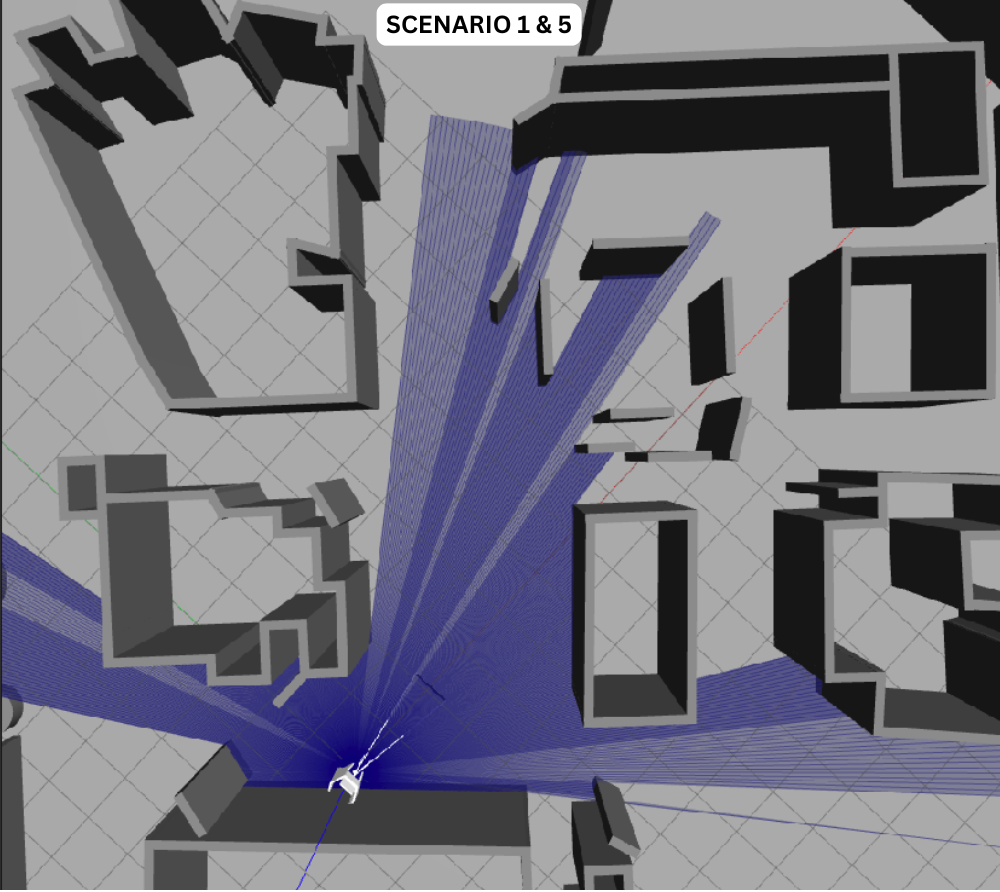
\includegraphics[width=\textwidth]{gambar/3.8_skenario_S1_S5.png}
        \\(a) S1/S5
    \end{minipage}
    \hfill
    \begin{minipage}{0.48\textwidth}
        \centering
        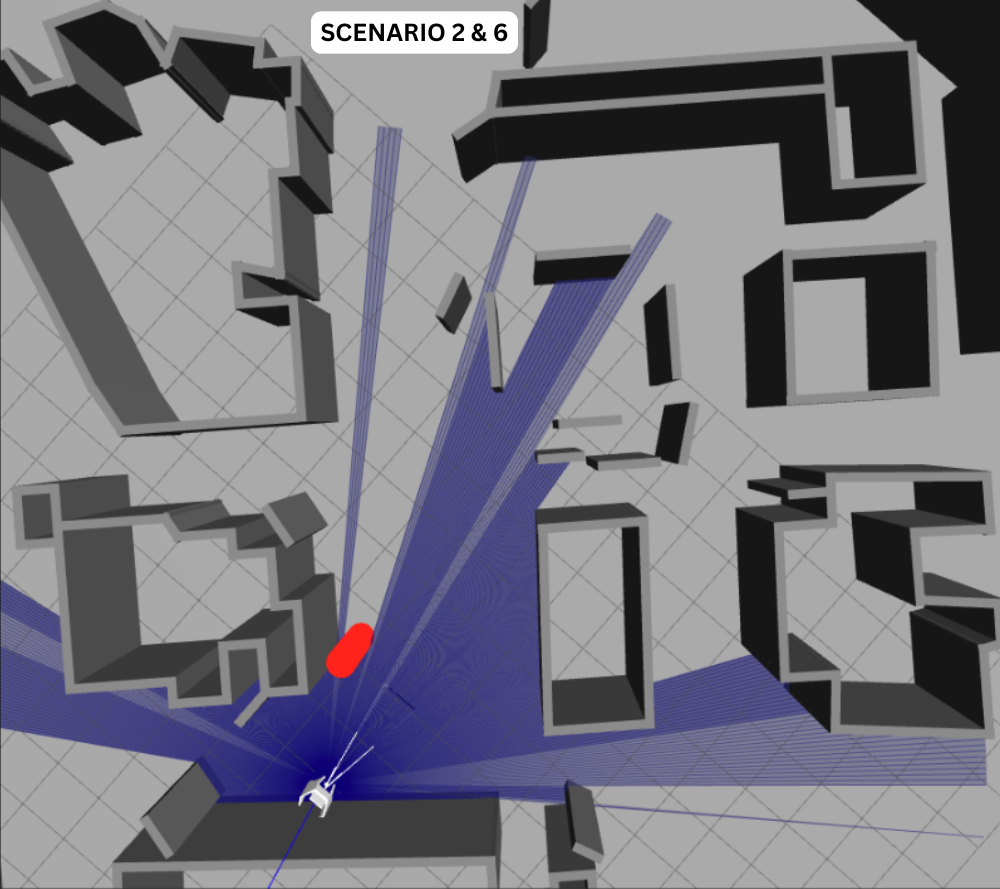
\includegraphics[width=\textwidth]{gambar/3.8_skenario_S2_S6.png}
        \\(b) S2/S6
    \end{minipage}

    \vspace{0.5em}

    \begin{minipage}{0.48\textwidth}
        \centering
        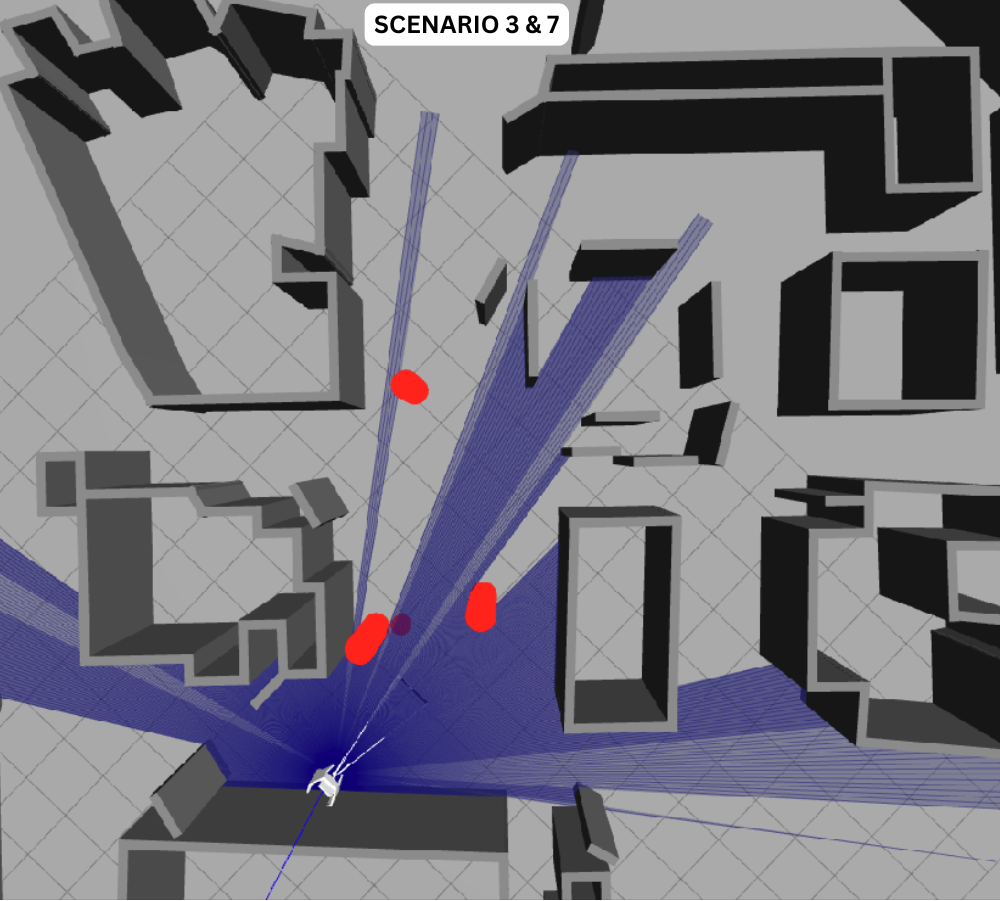
\includegraphics[width=\textwidth]{gambar/3.8_skenario_S3_S7.png}
        \\(c) S3/S7
    \end{minipage}
    \hfill
    \begin{minipage}{0.48\textwidth}
        \centering
        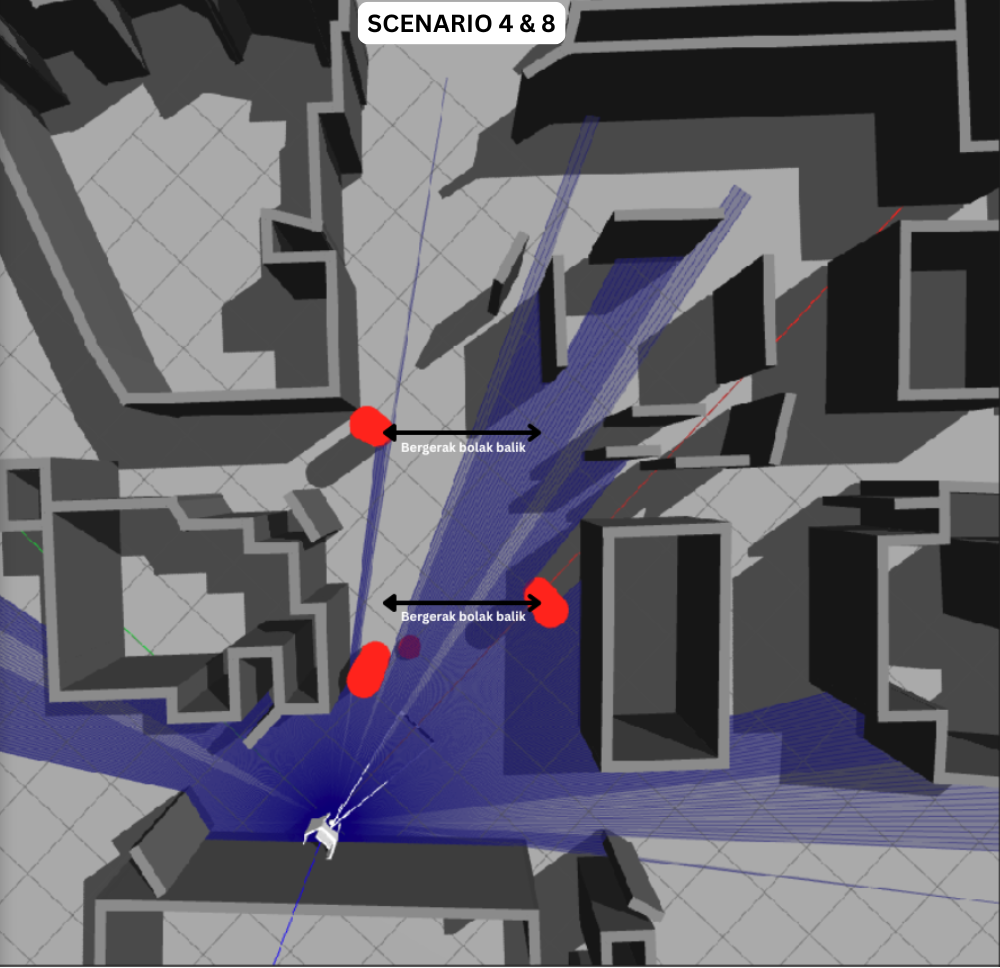
\includegraphics[width=\textwidth]{gambar/3.8_skenario_S4_S8.png}
        \\(d) S4/S8
    \end{minipage}
    \caption{Tampak atas empat lingkungan pengujian di Gazebo. Jalur biru menunjukkan jangkauan pindaian LiDAR \textit{real-time}; blob merah menandai sumber panas yang terdeteksi kamera termal. (a) S1/S5: tanpa \textit{obstacle} aktif. (b) S2/S6: satu \textit{obstacle} statis bersuhu tubuh. (c) S3/S7: tiga sumber panas (\textit{obstacle\_cat} dan dua \textit{obstacle\_human}) dari total empat \textit{obstacle} fisik; satu \textit{obstacle} statis tambahan tidak terdeteksi termal karena tidak bersuhu tubuh. (d) S4/S8: dua \textit{obstacle\_human} bergerak osilasi (ditandai panah \textit{"Bergerak bolak balik"}), sedangkan \textit{obstacle\_cat} tetap statis.}
    \label{fig:skenario_panel}
\end{figure}

\begin{figure}[H]
    \centering
    \begin{minipage}{0.48\textwidth}
        \centering
        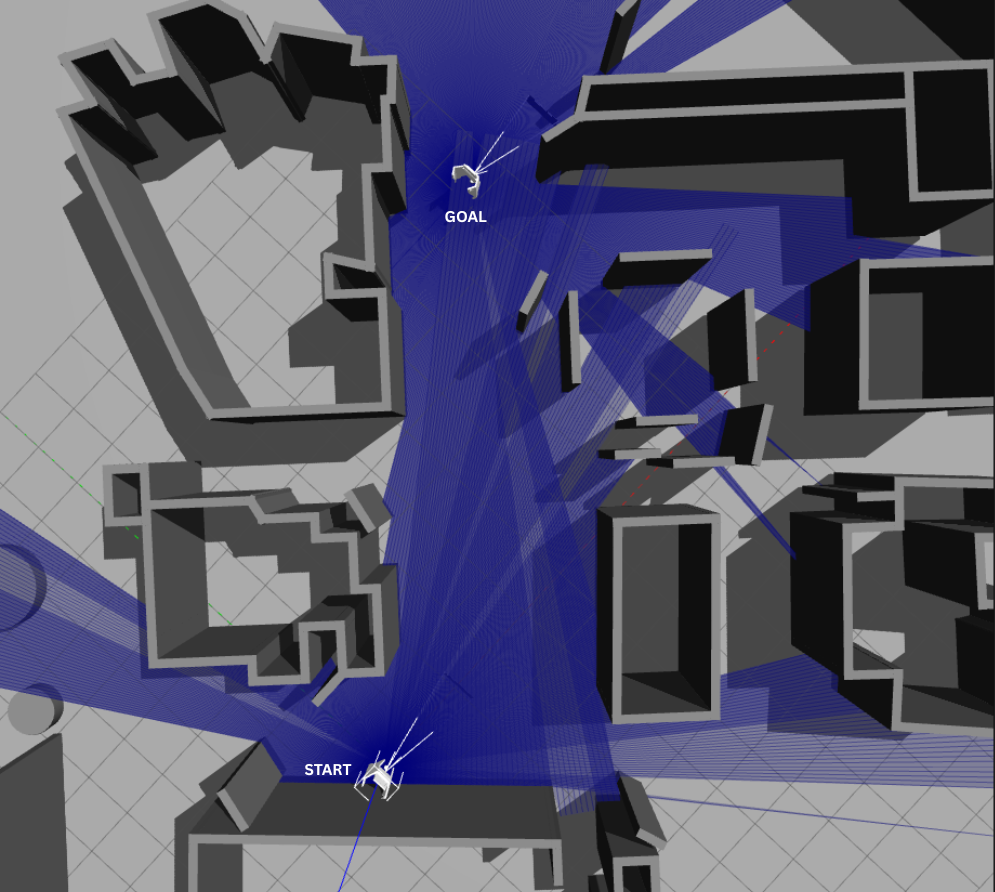
\includegraphics[width=\textwidth]{gambar/3.8_map_gazebo.png}
        \\(a) Tampak atas Gazebo
    \end{minipage}
    \hfill
    \begin{minipage}{0.48\textwidth}
        \centering
        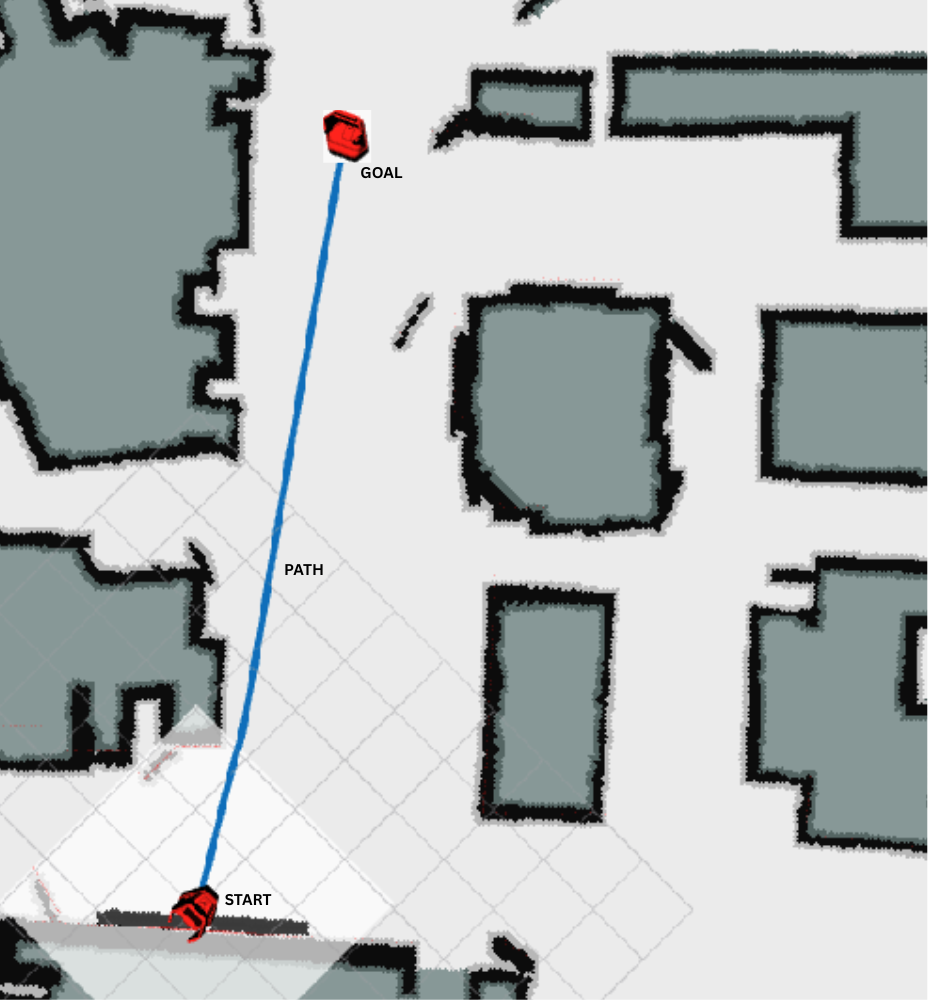
\includegraphics[width=\textwidth]{gambar/3.8_map_rviz.png}
        \\(b) Representasi RViz
    \end{minipage}
    \caption{Konfigurasi titik awal (START) dan tujuan (GOAL) yang identik untuk seluruh delapan skenario pengujian. (a) Tampak atas pada simulator Gazebo, menunjukkan kompleksitas geometris lingkungan \textit{indoor}. (b) Representasi pada RViz menggunakan peta \texttt{grit\_1\_edited\_2} (\textit{occupancy grid}), dengan garis biru menunjukkan jalur global yang dihasilkan NavfnROS sebelum eksekusi \textit{trial}. Koordinat \textit{frame} peta: START $= (0, 0)$, GOAL $= (9{,}159;\ 6{,}240)$.}
    \label{fig:map_annotated}
\end{figure}

Pada seluruh skenario, posisi awal robot ditetapkan pada koordinat yang sama, sedangkan posisi tujuan ditentukan pada titik akhir koridor navigasi. Dengan konfigurasi tersebut, seluruh percobaan dilakukan pada kondisi awal yang identik sehingga hasil pengujian dapat dibandingkan secara adil.

\subsection{Konfigurasi Baseline dan Fuzzy}

Konfigurasi baseline (S1--S4) menggunakan APFPlanner dengan parameter navigasi yang bersifat tetap. Pada konfigurasi ini, kecepatan robot dan penguatan gaya tolak obstacle dihitung menggunakan parameter bawaan APF tanpa mekanisme adaptasi.

Sebaliknya, konfigurasi fuzzy (S5--S8) menggunakan pengendali fuzzy Mamdani yang telah dijelaskan pada Subbab~\ref{sec:fuzzy_Aapf}. Nilai traversability efektif dan jarak obstacle terdekat digunakan sebagai masukan fuzzy untuk menghasilkan parameter \textit{speed scale} dan \textit{repulsive gain} secara adaptif.

Perbedaan utama kedua konfigurasi dirangkum pada Tabel~\ref{tab:konfigurasi_eksperimen}.

\begin{table}[H]
\centering
\caption{Perbandingan konfigurasi eksperimen}
\label{tab:konfigurasi_eksperimen}
\begin{tabular}{lll}
\toprule
\textbf{Komponen} &
\textbf{Baseline} &
\textbf{Fuzzy} \\
\midrule
LiDAR & Aktif & Aktif \\
Kamera termal & Aktif & Aktif \\
Virtual LaserScan & Aktif & Aktif \\
Fusi traversability & Aktif & Aktif \\
APFPlanner & Aktif & Aktif \\
Fuzzy Mamdani & Tidak aktif & Aktif \\
\bottomrule
\end{tabular}
\end{table}

\subsection{Prosedur Pelaksanaan Eksperimen}

Setiap skenario dieksekusi sebanyak sepuluh kali percobaan independen untuk memperoleh hasil yang lebih representatif dan mengurangi pengaruh variasi acak selama simulasi. Jumlah replikasi tersebut dipilih agar data yang diperoleh mencukupi untuk analisis statistik nonparametrik pada tahap evaluasi.

Urutan pelaksanaan eksperimen ditunjukkan pada Gambar~\ref{fig:prosedur_pengujian}.

\begin{figure}[H]
\centering
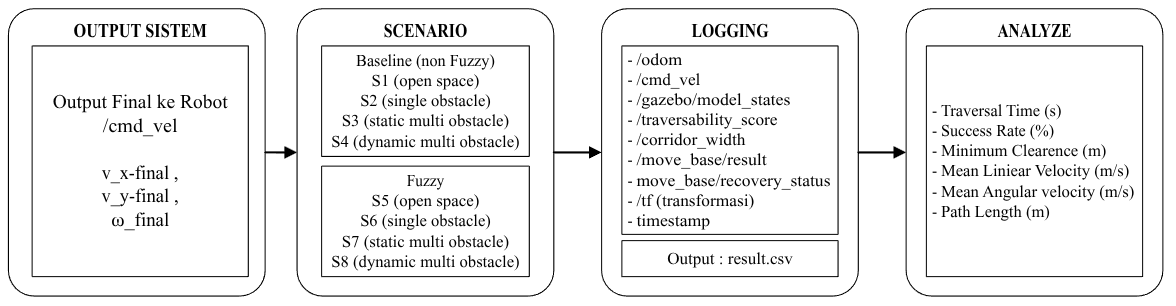
\includegraphics[width=0.9\textwidth]{gambar/3.8_prosedur_pengujian.png}
\caption{Alur pelaksanaan eksperimen.}
\label{fig:prosedur_pengujian}
\end{figure}

Secara umum, prosedur pengujian dilakukan melalui langkah-langkah berikut:

\begin{enumerate}
\item Menjalankan lingkungan simulasi Gazebo dan ROS.
\item Memuat peta navigasi dan model robot.
\item Mengaktifkan sensor LiDAR dan kamera termal.
\item Menjalankan modul navigasi sesuai konfigurasi pengujian.
\item Menetapkan posisi awal dan tujuan robot.
\item Menjalankan simulasi hingga robot mencapai tujuan atau eksperimen dihentikan.
\item Menyimpan seluruh data hasil eksperimen.
\item Mengulangi proses untuk seluruh skenario dan seluruh replikasi.
\end{enumerate}

\subsection{Pencatatan Data Eksperimen}

Selama eksperimen berlangsung, seluruh data dicatat secara otomatis menggunakan node \texttt{experiment\_logger.py}. Pencatatan dilakukan untuk memastikan seluruh informasi yang diperlukan pada tahap evaluasi tersedia secara lengkap dan konsisten.

Data yang direkam meliputi:

\begin{itemize}
\item posisi dan orientasi robot (\texttt{/odom}),
\item kecepatan linear dan angular (\texttt{/cmd\_vel}),
\item nilai traversability efektif,
\item jarak obstacle terdekat,
\item status pencapaian tujuan,
\item waktu pelaksanaan eksperimen.
\end{itemize}

Seluruh data disimpan dalam format CSV sehingga dapat digunakan untuk proses analisis statistik pada tahap berikutnya.

\section{Metode Evaluasi dan Analisis Data}
\label{sec:evaluasi}
Subbab ini menjelaskan metode evaluasi yang digunakan untuk menilai pengaruh integrasi kamera termal dan pengendali fuzzy terhadap performa sistem navigasi robot. Evaluasi difokuskan pada dua aspek utama, yaitu keamanan navigasi (\textit{safety}) dan efisiensi pergerakan (\textit{efficiency}). Seluruh metrik, prosedur pencatatan data, serta metode analisis statistik dirancang untuk mengevaluasi kontribusi sistem yang diusulkan secara objektif dan dapat direproduksi.

\subsection{Tujuan Evaluasi}

Tujuan evaluasi pada penelitian ini adalah menilai pengaruh integrasi kamera termal dan pengendali fuzzy terhadap performa navigasi robot pada berbagai kondisi lingkungan.

Evaluasi difokuskan pada empat aspek utama, yaitu:

\begin{enumerate}
\item kemampuan menghindari obstacle pada area \textit{blind-spot} LiDAR;
\item peningkatan margin keselamatan navigasi yang direpresentasikan oleh nilai \textit{minimum clearance};
\item pengaruh metode usulan terhadap efisiensi navigasi;
\item pengaruh metode usulan terhadap stabilitas dan kehalusan pergerakan robot.
\end{enumerate}

\subsection{Metrik Evaluasi}
\label{sec:metrik}

Kinerja sistem dinilai menggunakan beberapa metrik yang mewakili aspek keamanan, efisiensi, dan kualitas pergerakan robot. Seluruh metrik direkam secara otomatis menggunakan \texttt{experiment\_logger.py} selama eksperimen berlangsung.

\subsubsection*{a. Tingkat Keberhasilan Navigasi (\textit{Success Rate})}

Sebuah \textit{trial} dinyatakan berhasil apabila robot mencapai tujuan dalam batas waktu pengujian dan tidak mengalami tabrakan selama perjalanan.

\begin{equation}
success=
\begin{cases}
1, & \text{jika } goal\_reached = 1 \\
   & \text{dan } collision\_count = 0 \\
   & \text{dan } t \leq 120\ \text{s} \\
0, & \text{lainnya}
\end{cases}
\label{eq:success}
\end{equation}

Tingkat keberhasilan dihitung menggunakan:

\begin{equation}
SR=
\frac{\sum success}{n}\times100\%
\label{eq:success_rate}
\end{equation}

dengan $n$ adalah jumlah \textit{trial} pada setiap skenario.

Selain itu, keamanan navigasi juga dievaluasi menggunakan \textit{Collision-Free Rate} (CFR), yaitu persentase percobaan yang tidak mengalami tabrakan selama proses navigasi berlangsung.

\begin{equation}
CFR=
\frac{\sum collision\_free}{n}\times100\%
\label{eq:cfr}
\end{equation}

Nilai CFR yang tinggi menunjukkan kemampuan sistem dalam mempertahankan navigasi bebas tabrakan.

\subsubsection*{b. Minimum Clearance}

\textit{Clearance} merepresentasikan jarak bebas antara robot dan obstacle selama navigasi. Untuk setiap obstacle yang diamati, nilai clearance dihitung sebagai:

\begin{equation}
c_{i,k}
=
d_{i,k}
-
r_{robot}
-
r_{obs,k}
\label{eq:clearance}
\end{equation}

dengan:

\begin{itemize}
\item $d_{i,k}$ adalah jarak pusat robot terhadap obstacle ke-$k$,
\item $r_{robot}$ adalah radius robot,
\item $r_{obs,k}$ adalah radius obstacle ke-$k$.
\end{itemize}

Nilai minimum clearance selama satu \textit{trial} dihitung sebagai:

\begin{equation}
c_{min}
=
\min(c_{i,k})
\label{eq:min_clearance}
\end{equation}

Minimum clearance dipilih sebagai metrik utama karena secara langsung merepresentasikan margin keselamatan yang dipertahankan robot terhadap obstacle selama proses navigasi berlangsung. Berbeda dengan \textit{success rate} yang hanya menunjukkan hasil akhir navigasi, minimum clearance mampu menggambarkan tingkat risiko kolisi yang dialami robot sepanjang lintasan yang ditempuh. Metrik ini menjadi sangat relevan karena tujuan utama integrasi kamera termal dan pengendali fuzzy adalah meningkatkan kemampuan robot dalam mempertahankan jarak aman terhadap obstacle, khususnya obstacle berprofil rendah yang berada pada area \textit{blind-spot} LiDAR.

\subsubsection*{c. Waktu Navigasi}

Waktu navigasi menunjukkan durasi yang dibutuhkan robot untuk mencapai tujuan.

\begin{equation}
t_{nav}
=
t_{finish}
-
t_{start}
\label{eq:nav_time}
\end{equation}

Metrik ini digunakan untuk mengevaluasi efisiensi temporal sistem navigasi.

\subsubsection*{d. Panjang Lintasan}

Panjang lintasan dihitung dari trajektori robot yang diperoleh melalui data odometri.

\begin{equation}
L
=
\sum_{i=1}^{N}
\sqrt{
(x_i-x_{i-1})^2
+
(y_i-y_{i-1})^2
}
\label{eq:path_length}
\end{equation}

Nilai yang lebih kecil menunjukkan jalur yang lebih efisien.

\subsubsection*{e. Kecepatan Rata-Rata}

Kecepatan linear rata-rata dihitung menggunakan:

\begin{equation}
\bar{v}
=
\frac{1}{N}
\sum_{i=1}^{N}
|v_i|
\label{eq:avg_linear}
\end{equation}

sedangkan kecepatan angular rata-rata dihitung menggunakan:

\begin{equation}
\bar{\omega}
=
\frac{1}{N}
\sum_{i=1}^{N}
|\omega_i|
\label{eq:avg_angular}
\end{equation}

Nilai $\bar{\omega}$ digunakan sebagai indikator kehalusan pergerakan robot selama navigasi.

\begin{table}[H]
\centering
\caption{Ringkasan metrik evaluasi}
\label{tab:metrik}
\begin{tabular}{llll}
\toprule
\textbf{Metrik} &
\textbf{Simbol} &
\textbf{Satuan} &
\textbf{Dimensi} \\
\midrule
Success Rate & $SR$ & \% & Efisiensi \\
Collision-Free Rate & $CFR$ & \% & Keamanan \\
Minimum Clearance & $c_{min}$ & m & Keamanan \\
Waktu Navigasi & $t_{nav}$ & s & Efisiensi \\
Panjang Lintasan & $L$ & m & Efisiensi \\
Kecepatan Linear Rata-rata & $\bar{v}$ & m/s & Kualitas \\
Kecepatan Angular Rata-rata & $\bar{\omega}$ & rad/s & Kehalusan \\
\bottomrule
\end{tabular}
\end{table}

\begin{table}[H]
\centering
\caption{Hubungan metrik evaluasi dan tujuan analisis}
\label{tab:metric_mapping}
\begin{tabular}{lll}
\toprule
\textbf{Tujuan Evaluasi} &
\textbf{Metrik} &
\textbf{Bab IV} \\
\midrule
Keselamatan Navigasi &
Minimum Clearance &
4.4 \\
Keberhasilan Navigasi &
Success Rate, CFR &
4.3 \\
Efisiensi Navigasi &
Navigation Time, Path Length &
4.5 \\
Kehalusan Gerak &
Average Angular Velocity &
4.6 \\
\bottomrule
\end{tabular}
\end{table}

\subsection{Akuisisi dan Logging Data}

Pencatatan data dilakukan secara otomatis menggunakan node \texttt{experiment\_logger.py}. Node ini berjalan selama eksperimen berlangsung dan merekam seluruh data yang diperlukan untuk proses evaluasi.

Topik yang digunakan selama proses logging meliputi:

\begin{itemize}
\item \texttt{/odom},
\item \texttt{/cmd\_vel},
\item \texttt{/gazebo/model\_states},
\item \texttt{/move\_base/result},
\item \texttt{/move\_base/recovery\_status},
\item \texttt{/traversability\_score},
\item \texttt{/corridor\_width}.
\end{itemize}

Pada akhir setiap \textit{trial}, seluruh metrik disimpan ke berkas CSV pada direktori \texttt{experime\-nt\_data}. Selain ringkasan metrik, trajektori robot juga disimpan untuk keperluan visualisasi dan analisis lebih lanjut pada Bab~IV.

\subsection{Analisis Statistik}

\subsubsection*{a. Pemilihan Uji Statistik}

Setiap skenario dieksekusi sebanyak sepuluh kali percobaan independen. Dengan ukuran sampel yang relatif kecil ($n = 10$ per kelompok), asumsi distribusi normal tidak dapat dijamin. Oleh karena itu, penelitian ini menggunakan uji non-parametrik Mann--Whitney U yang tidak mensyaratkan distribusi normal dan banyak digunakan pada evaluasi sistem robotika berbasis simulasi (\cite{Adiuku2024}).

\subsubsection*{b. Uji Mann--Whitney U}

Analisis dilakukan secara berpasangan pada S1--S5, S2--S6, S3--S7, dan S4--S8.

Hipotesis statistik yang digunakan adalah:

\begin{itemize}
\item $H_0$: distribusi kedua kelompok identik.
\item $H_1$: terdapat perbedaan distribusi antara kedua kelompok.
\end{itemize}

Tingkat signifikansi yang digunakan adalah:

\begin{equation}
\alpha = 0.05
\end{equation}

\subsubsection*{c. Effect Size}

Selain signifikansi statistik, penelitian ini menghitung \textit{effect size} menggunakan \textit{rank-bise\-rial correlation} (\cite{Kerby2014}):

\begin{equation}
r
=
1 - \frac{2U}{n_1 n_2}
\label{eq:rank_biserial}
\end{equation}

dengan $U$ adalah statistik Mann--Whitney dan $n_1$ serta $n_2$ adalah ukuran sampel masing-masing kelompok.

Interpretasi nilai \textit{rank-biserial correlation} mengacu pada pedoman umum yang mengelompokkan nilai absolut koefisien menjadi efek kecil ($|r| < 0{,}30$), efek sedang ($0{,}30 \leq |r| < 0{,}50$), dan efek besar ($|r| \geq 0{,}50$). Nilai positif menunjukkan bahwa kelompok fuzzy cenderung menghasilkan nilai metrik yang lebih tinggi dibandingkan kelompok \textit{baseline}, sedangkan nilai negatif menunjukkan kecenderungan sebaliknya.

\subsection{Interpretasi Hasil}

Analisis hasil pada Bab~IV difokuskan pada empat aspek utama, yaitu:

\begin{enumerate}
\item peningkatan keamanan navigasi melalui \textit{minimum clearance};
\item kemampuan menghindari obstacle pada area \textit{blind-spot} LiDAR;
\item efisiensi navigasi berdasarkan waktu tempuh dan panjang lintasan;
\item kualitas pergerakan berdasarkan karakteristik kecepatan robot.
\end{enumerate}

Hasil pengujian disajikan dalam bentuk tabel statistik, grafik distribusi data, visualisasi trajektori, serta analisis perbandingan antara konfigurasi \textit{baseline} dan fuzzy pada setiap skenario pengujian.
